% Generational Depth Estimation
\documentclass[11pt]{article}
\usepackage[review]{acl}
\usepackage{times}
\usepackage{latexsym}
\usepackage[T1]{fontenc}
\usepackage[utf8]{inputenc}
\usepackage{microtype}
\usepackage{graphicx}
\usepackage{amsmath}
\usepackage{amssymb}
\usepackage{booktabs}
\usepackage{colortbl}
\usepackage{multirow}
\usepackage{enumitem}
\usepackage{subcaption}
\usepackage{placeins}
\usepackage{float}

\newcommand{\Kstar}{{K^*}}
\newcommand{\Kempirical}{{K^*_{\text{empirical}}}}
\newcommand{\Ktheory}{{K^*_{\text{theory}}}}
\newcommand{\auc}{\text{AUC}}
\newcommand{\jsd}{\text{JSD}}

\title{Generational Depth Estimation of Recursive Synthetic Text:\\Measuring the Discrimination Boundary}

\author{Anonymous}

\begin{document}
\maketitle

% === Abstract ===
\begin{abstract}
Web-scale corpora are increasingly contaminated by recursive synthetic content, yet no method estimates a document's generational depth.
We measure a lower bound on the generational discrimination boundary, $\Kempirical$ (the maximum depth at which adjacent generations remain distinguishable).
Under prompt-chain generation across 10 model configurations (6 architecture families, 1B--8B), 4 source domains, and 4 decoding strategies, $\Kempirical \leq 2$ for all web text configurations (discrimination threshold $\theta{=}0.60$); structured academic text (arXiv) reaches $\Kempirical{=}3$ across four independent architecture families.
Beyond two generation passes, web text becomes statistically indistinguishable across deeper generations, a \emph{one-wash laundering} effect that concentrates the dominant exploitable signal at the human-vs.-machine boundary.
Across continuation-mode generators, generator-agnostic statistical features enable 80--92\% cross-model transfer with scorer-invariant feature rankings ($\rho > 0.90$); depth estimation on corpora from unknown generators requires no retraining.
Under extreme contamination (${\sim}$83\% synthetic), $\Kempirical$ correctly predicts that binary filtering outperforms graduated alternatives; at realistic ratios ($\leq$50\%), strategy differences remain below 0.3\,pp\footnote{Code and data are available at \url{https://anonymous.4open.science/r/gen-depth-contamination-E6C1/}.}.
\end{abstract}

% === Section 1: Introduction ===
\section{Introduction}
\label{sec:introduction}

Web-scale text corpora are increasingly contaminated by synthetic content that has itself been generated from earlier synthetic content.
Estimates suggest that a substantial fraction of online text is machine-generated~\cite{sun2025aigt, spennemann2025quantifying}, and this share continues to rise.
When models train on the outputs of earlier models, the resulting multi-generational synthetic text degrades with each iteration: tail modes vanish, lexical diversity contracts, and surprisal distributions flatten~\cite{shumailov2024collapse, dohmatob2024model}.
This degradation arises in both \emph{retrain-chains} (iteratively training on model outputs) and \emph{prompt-chains} (recursively generating from previous outputs without retraining); we study the latter, which isolates generation-level information loss from training dynamics (Appendix~\ref{sec:extended_limitations}).
Yet the dominant paradigm treats all machine-generated text identically, discarding the generational depth dimension.

This gap cuts across four lines of work: binary detectors~\cite{basani2026diveye, zhang2024minkpp} produce no depth estimate (Section~\ref{sec:binary_confidence}); membership inference~\cite{zawalski2026codec} addresses a different question; the model collapse literature~\cite{shumailov2024collapse, alemohammad2024selfconsuming, schaeffer2025position} provides no per-text tool; and data selection methods~\cite{xie2023dsir, tirumala2023d4, drayson2025} ignore recursive depth.
No existing method estimates how many rounds of recursive generation a text has undergone.

The Data Processing Inequality guarantees that information degrades monotonically across generations, motivating a finite discrimination boundary $\Kstar$.
We empirically measure a lower bound $\Kempirical$ on the discrimination boundary (the maximum depth at which a classifier reliably distinguishes adjacent generations) using 15 statistical features and an Ordinal Binary Decomposition (OBD) LightGBM classifier.
We operationalize $\Kempirical$ as the deepest $k \geq 1$ where the pairwise area under the ROC curve ($\auc_{k-1,k}$) exceeds $\theta = 0.60$ (Section~\ref{sec:formulation}).

Our contributions:
\begin{enumerate}[label=(\alph*),nosep]
  \item \textbf{Measuring the discrimination boundary}: $\Kempirical \leq 2$ across all 10 model configurations (6 architecture families at 1B--8B scale) and 4 decoding strategies; $\Kempirical{=}2$ for 6/10 spanning three families ($p < 0.001$; Section~\ref{sec:kstar_boundary}).
  Beyond two generation passes, web text becomes statistically indistinguishable across deeper generations; this finding establishes binary sufficiency by measurement, reveals domain-dependent variation (arXiv $\Kempirical{=}3$), and quantifies boundary sensitivity to threshold, scorer, and scale.
  Both supervised OBD and zero-shot large language models (LLMs) fail beyond $\Kempirical$ (McNemar $p > 0.05$; Section~\ref{sec:why_kstar}).
  \item \textbf{Domain dependence of $\Kempirical$}: general web text (C4, Wikipedia) and code yield $\Kempirical{\leq}2$, while structured academic text (arXiv) yields $\Kempirical{=}3$, consistent across model families (Section~\ref{sec:cross_domain}).
  \item \textbf{Generator-agnostic cross-model transfer} (within continuation mode): 15 statistical features enable 80--92\% accuracy retention with scorer-invariant feature rankings ($\rho > 0.90$), supporting depth estimation on corpora from unknown continuation-mode generators without retraining; $\Kempirical$ agreement holds across scorers for strong-signal configurations (Section~\ref{sec:transfer}).
\end{enumerate}

\noindent As a consistency check under extreme contamination (${\sim}$83\% synthetic), $\Kempirical{=}2$ correctly predicts the strategy ordering: binary curation minimizes Massive Multitask Language Understanding (MMLU) degradation ($0.5941$ vs.\ base $0.6018$); at realistic ratios ($\leq$50\%), all strategies converge (Section~\ref{sec:filtering}).


% === Section 2: Related Work ===
\section{Related Work}
\label{sec:related_work}

\paragraph{Model collapse and recursive degradation.}
Iterative training on model outputs causes tail-distribution degradation~\cite{shumailov2024collapse, alemohammad2024selfconsuming, dohmatob2024model, dohmatob2025strong}, diversity contraction~\cite{guo2024curious, padmakumar2024writing, briesch2023selfconsuming}, and predictable convergence dynamics~\cite{schaeffer2025position, kazdan2025collapse, gerstgrasser2024model, wang2025unveiling}.
Fu et al.~\cite{fu2025theoretical} formalize the convergence via Markov chain theory, complementing the DPI's mutual information monotonicity.
Our prompt-chain operates in the replace regime~\cite{kazdan2025collapse}, making $\Kempirical = 2$ a conservative lower bound; empirically, detection accuracy erodes with each generation~\cite{hao2025rewrite}, consistent with our measured discrimination boundary.
This literature characterizes macro dynamics but provides no per-text depth estimation, the gap we address.

\paragraph{Machine-generated text detection.}
Statistical detectors~\cite{mitchell2023detectgpt, bao2024fast} and model-based classifiers~\cite{hans2024binoculars, basani2026diveye, zhang2024minkpp, verma2024ghostbuster} achieve strong human-vs.-machine separation; benchmarks such as RAID~\cite{dugan2024raid} evaluate robustness at scale.
Recent extensions move beyond binary labels: Cheng et al.~\cite{cheng2025beyond} estimate human-AI collaboration degree, Mehta et al.~\cite{mehta2025beyond} propose contamination hierarchies, and Wang et al.~\cite{wang2024semeval} construct multigenerator benchmarks.
Robustness concerns arise under paraphrasing~\cite{sadasivan2023detect, krishna2023paraphrasing}, cross-mode transfer~\cite{hao2025rewrite}, and demographic bias~\cite{liang2023gpt}; CoDeC~\cite{zawalski2026codec} addresses contamination via membership inference.
None of these methods estimates recursive generation depth.

\paragraph{Data curation, ordinal methods, and watermarking.}
Data Selection with Importance Resampling (DSIR)~\cite{xie2023dsir}, D4~\cite{tirumala2023d4}, and DoReMi~\cite{xie2023doremi} select training data by domain relevance but are depth-agnostic; Drayson et al.~\cite{drayson2025} combined binary detection with importance resampling, a special case when $\Kstar = 1$.
Our OBD classifier follows Frank \& Hall's~\cite{frank2001ordinal} binary decomposition for ordinal regression; our neural probe extends probing~\cite{alain2017understanding, belinkov2022probing} to the discrimination boundary.
Text watermarking~\cite{kirchenbauer2023watermark} embeds provenance signals proactively; our work addresses the complementary post-hoc scenario where the generator is not controlled.


% === Section 3: Method ===
\section{Method}
\label{sec:method}

\begin{figure*}[t]
\centering
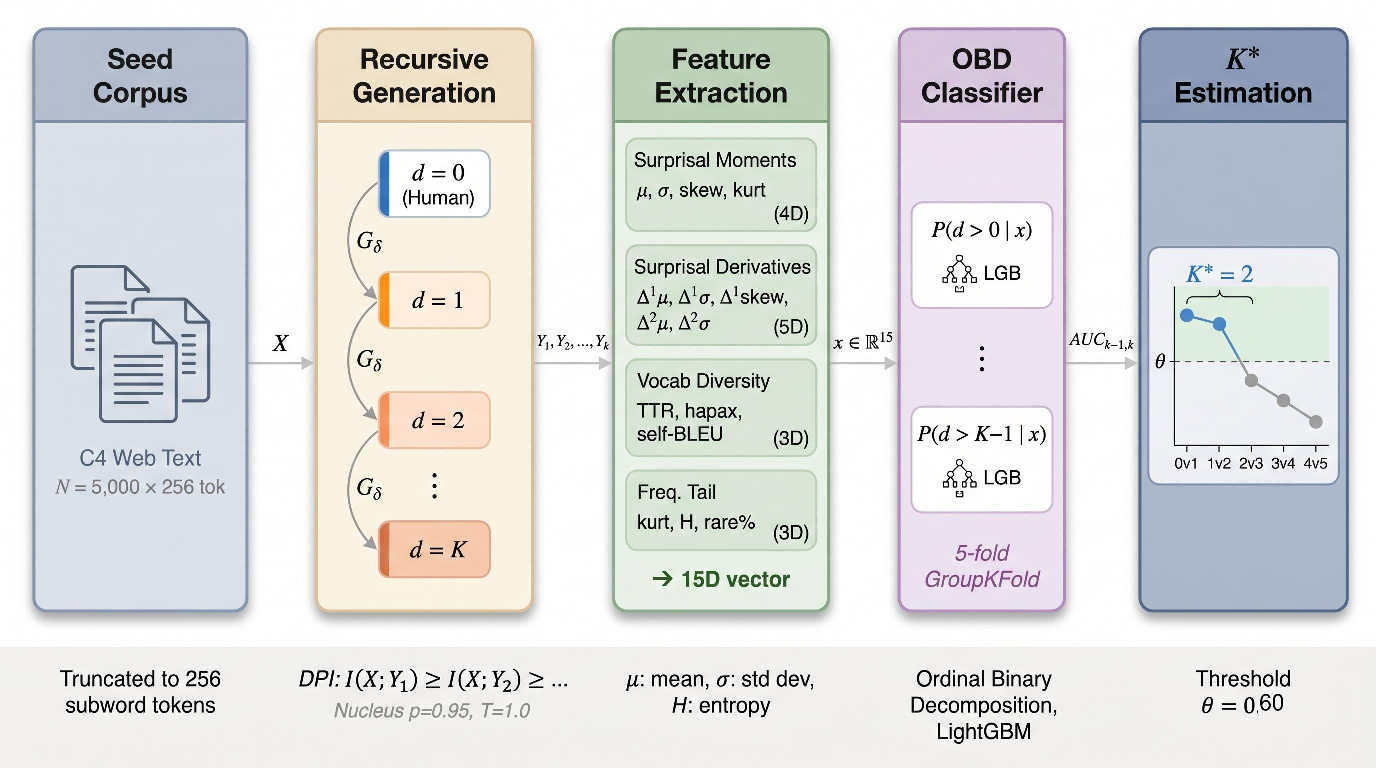
\includegraphics[width=\textwidth]{figures/pipeline.pdf}
\caption{Generational depth estimation pipeline. Seed documents are recursively passed through a generation operator $G_\delta$ to produce a depth chain. Corpus-level statistical features are fed to the OBD-LightGBM classifier for depth prediction. (Simplified notation; see Eq.~\ref{eq:kstar} for the formal $\Kempirical$ definition.)}
\label{fig:pipeline}
\end{figure*}

\subsection{Problem Formulation}
\label{sec:formulation}

A generation operator $G_\delta$ (LLM + decoding strategy $\delta$) produces successive generations $X \to Y_1 \to \cdots \to Y_K$, where $Y_k = G_\delta(Y_{k-1})$ and $Y_0 \triangleq X$ (Figure~\ref{fig:pipeline}).
This sequence forms a Markov chain.
By the Data Processing Inequality, $I(X; Y_1) \geq I(X; Y_2) \geq \cdots \geq 0$: mutual information with the seed text degrades monotonically.
Together with Markov chain convergence, this motivates the existence of a finite discrimination boundary where $\auc_{k-1,k}$ falls below a decision threshold, though AUC and mutual information are not formally equivalent; the actual saturation depth must therefore be measured empirically.
Pairwise AUC generally decreases with depth but may exhibit noise-level reversals (e.g., Pythia-1.4B 3v4 $\auc = 0.505$ vs.\ 4v5 $= 0.508$, a difference within bootstrap CI; Table~\ref{tab:kstar_ci_extended}), reinforcing that $\Kempirical$ is a measured quantity rather than a theoretical prediction.

We define the operational lower bound:
{\small
\begin{equation}
  \Kempirical = \max\bigl\{k \!\geq\! 1 : \auc_{j-1,j} > \theta,\;\forall\, 1 \!\leq\! j \!\leq\! k\bigr\},
  \label{eq:kstar}
\end{equation}
}
which requires all pairs up to depth $k$ to exceed the threshold (the $\forall j$ constraint is naturally satisfied because $\auc_{k-1,k}$ decreases monotonically above $\theta$ across all tested configurations; Table~\ref{tab:kstar_ci}).
The theoretical upper bound $\Ktheory$ (the true maximum discriminable depth given optimal features) is not directly estimated in this work.
Since any specific classifier on a feature subset achieves AUC at most equal to the Bayes-optimal classifier on all features, $\Kempirical \leq \Ktheory$ follows directly.
The DPI motivates the empirical observation that $\auc_{k-1,k}$ generally decreases with $k$ under non-degenerate decoding, though AUC is not a monotone function of MI (as noted above).
Here $\auc_{k-1,k}$ is the point-estimate pairwise AUC and $\theta = 0.60$ is a reference operating point; $\theta$ sits between the 1v2 AUC cluster ($0.607$--$0.696$) and the 2v3 cluster ($0.55$--$0.59$), so that $\Kempirical$ is insensitive to the exact threshold within this range (justified below; Figure~\ref{fig:kstar_theta}).
All pairwise significance tests use 10{,}000-iteration permutation tests with Bonferroni correction for 10 comparisons ($\alpha_{\text{corrected}}{=}0.005$); we report bootstrap 95\% confidence intervals (CIs) (1{,}000 resamples unless otherwise noted) for all boundary-pair AUCs and explicitly mark marginal cases where Bonferroni-corrected lower bounds fall below $\theta$ (Section~\ref{sec:kstar_boundary}).

\paragraph{Threshold justification.}
$\theta{=}0.60$ is a reference operating point supported by two independent lines of evidence.
First, a 10{,}000-iteration permutation test yields a 95th-percentile null of ${<}\,0.55$ ($p < 0.002$ for all boundary comparisons).
Second, $\Kempirical{=}2$ is insensitive to the exact threshold: 1v2 AUC values cluster at $0.607$--$0.696$ while 2v3 values cluster at $0.55$--$0.59$, a ${\sim}$1--10\,pp discontinuity that ensures $\Kempirical$ is stable across $\theta \in [0.59, 0.60]$; at $\theta{=}0.61$, one borderline case (Pythia-1.4B, 1v2 $\auc{=}0.607$) shifts to $\Kempirical{=}1$.
Only at extremes does $\Kempirical$ shift broadly ($\theta{=}0.55$: $\Kempirical{=}3$ for two Qwen configurations; $\theta{=}0.70$: $\Kempirical{=}1$ across all).
Figure~\ref{fig:kstar_theta} provides the full sensitivity surface across $\theta \in [0.50, 0.70]$.
The downstream filtering evaluation (Section~\ref{sec:filtering}) uses the OBD classifier without re-optimizing $\theta$, avoiding circularity.

\subsection{Features and Classifier}
\label{sec:features}

Each document is characterized by a 15-dimensional feature vector spanning four groups: \emph{surprisal moments} (mean, std, skewness, kurtosis; 4~dims), \emph{surprisal derivatives} (mean and std of first- and second-order differences, plus first-order skewness; 5~dims), \emph{vocabulary diversity} (type-token ratio (TTR), hapax legomena ratio, self-BLEU; 3~dims), and \emph{frequency tail statistics} (frequency kurtosis, entropy, rare token fraction; 3~dims).
All features are computed from token-level surprisal values via an external scorer model (full definitions in Table~\ref{tab:s5_features}, Appendix).
Self-BLEU reference sets are drawn exclusively within each fold to prevent information leakage across cross-validation splits; self-BLEU ranks \#1 in 1/8 conditions (greedy decoding) but is absent from the top-3 in all 7 others.
Removing self-BLEU reduces mean $\auc_{1v2}$ by $< 1$\,pp across all models (14D $\Kempirical = 2$ for all 4 configurations); in deployment where reference corpora are unavailable, self-BLEU can be replaced with corpus-level self-similarity or omitted entirely, leaving 14 features (surprisal statistics, TTR, hapax ratio, frequency tail) that require no external reference and retain full $\Kempirical$.
These features are generator-agnostic in that they require no knowledge of or access to the generating model, though they depend on an external scorer for surprisal computation (Section~\ref{sec:transfer}).

We use \emph{Ordinal Binary Decomposition} (OBD), decomposing the $(K{+}1)$-class problem into $K$ cumulative binary sub-classifiers, each estimating $P(\text{depth} > k \mid \mathbf{x})$ via LightGBM (hyperparameters in Table~\ref{tab:s6_lgbm_params}).
OBD achieves lower mean absolute error (MAE) than multiclass LightGBM (e.g., 0.984 vs.\ 1.016 on Qwen-rewrite) while maintaining superior pairwise $\auc$ (mean 0.6095 vs.\ 0.4883 for ordinal logistic regression) (Appendix~\ref{sec:computation_cost}).

\subsection{Experimental Setup}
\label{sec:experimental_setup}

We evaluate six primary configurations spanning three model families (Table~\ref{tab:setup}): Qwen2.5-1.5B-Instruct (rewrite and continuation), Qwen2.5-1.5B (base), Qwen2.5-7B, Pythia-1.4B, and OLMo-1B; four additional models are introduced in Section~\ref{sec:experiments}.
Each uses 5{,}000 C4 seeds truncated to 256 tokens, recursively generated for $K{=}5$ iterations (30{,}000 documents per configuration; Table~\ref{tab:s4_dataset_stats}).
Default decoding: nucleus $p{=}0.95$, $T{=}1.0$; decoding ablation covers greedy, nucleus $p{=}0.9$, $T{=}0.7$, and $T{=}1.2$.
Continuation mode truncates seeds to 128 tokens and extends to 256; rewrite mode paraphrases the full text.
Evaluation: 5-fold GroupKFold cross-validation grouped by seed document; pairwise $\auc$ as primary metric.

\begin{table}[t]
\centering
\small
\caption{Experimental configurations for depth-chain generation. \textbf{Config}: shorthand identifier; \textbf{Model}: architecture and parameter count; \textbf{Mode}: generation strategy (continuation or rewrite); $N$: number of seed documents per depth level.}
\label{tab:setup}
\begin{tabular}{llcc}
\toprule
\textbf{Config} & \textbf{Model} & \textbf{Mode} & $N$ \\
\midrule
Qwen-rw   & Qwen2.5-1.5B-Instruct & Rewrite & 5{,}000 \\
Qwen-cont & Qwen2.5-1.5B-Instruct & Continuation & 5{,}000 \\
Qwen-base & Qwen2.5-1.5B          & Continuation & 5{,}000 \\
Pythia    & Pythia-1.4B            & Continuation & 5{,}000 \\
OLMo      & OLMo-1B               & Continuation & 5{,}000 \\
Qwen-7B   & Qwen2.5-7B            & Continuation & 5{,}000 \\
\bottomrule
\end{tabular}
\end{table}


% === Section 4: Experiments ===
\section{Experiments}
\label{sec:experiments}

We evaluate on ten configurations spanning six families: Pythia-1.4B/6.9B, OLMo-1B, Qwen2.5-1.5B-Instruct (rewrite/continuation), Qwen2.5-1.5B (base), Qwen2.5-7B, LLaMA-3.1-8B, Mistral-7B, and Gemma-2-2B.
Unless noted, all experiments use the OBD-LightGBM classifier with 15 features (Section~\ref{sec:method}), 5{,}000 C4 texts per depth level (depths 0--5).

%% ====================================================================
\subsection{The Discrimination Boundary}
\label{sec:kstar_boundary}

\begin{figure}[t]
\centering
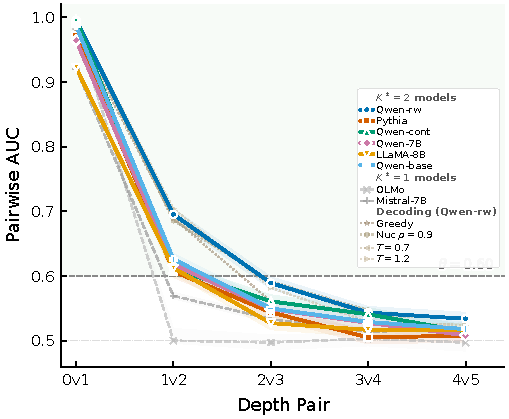
\includegraphics[width=\columnwidth]{figures/fig2_auc_decay.pdf}
\caption{Pairwise $\auc$ decay across adjacent depth pairs (0v1, 1v2, \ldots, 4v5) for model-mode configurations (solid) and decoding strategies (dashed); shaded bands show bootstrap 95\% CIs. Horizontal dashed line: $\theta = 0.60$.}
\label{fig:auc_decay}
\end{figure}

\begin{table*}[t]
\centering
\small
\caption{Pairwise $\auc$ for adjacent depth pairs with bootstrap 95\% CIs and permutation $p$-values for boundary rows.
$\Kempirical = 2$ requires 1v2 $\auc > \theta{=}0.60$ and 2v3 $\auc < \theta$; CIs quantify boundary uncertainty.
Extended results (all models) in Table~\ref{tab:kstar_ci_extended}.}
\label{tab:kstar_ci}
\resizebox{\textwidth}{!}{%
\begin{tabular}{lcccccccccc}
\toprule
 & \multicolumn{2}{c}{Qwen-rw} & \multicolumn{2}{c}{Pythia} & \multicolumn{2}{c}{OLMo} & \multicolumn{2}{c}{Qwen-cont} & \multicolumn{2}{c}{Qwen-7B\rlap{$^\ddagger$}} \\
\cmidrule(lr){2-3}\cmidrule(lr){4-5}\cmidrule(lr){6-7}\cmidrule(lr){8-9}\cmidrule(lr){10-11}
 & $\auc$ & 95\% CI & $\auc$ & 95\% CI & $\auc$ & 95\% CI & $\auc$ & 95\% CI & $\auc$ & 95\% CI \\
\midrule
0v1 & .9956 & & .9722 & & .9861 & & .9971 & & .9644 & [.961,\,.967] \\
1v2 & .6955 & [.686,\,.704]\rlap{$^*$} & .6074 & [.598,\,.617]\rlap{$^*$} & .5001 & [.496,\,.519] & .6112 & [.602,\,.621]\rlap{$^*$} & .6178 & [.608,\,.626]\rlap{$^*$} \\
2v3 & .5893 & [.580,\,.599] & .5440 & [.534,\,.554] & .4973 & [.486,\,.509] & .5609 & [.551,\,.571] & .5492 & [.539,\,.559] \\
3v4 & .5435 & & .5051 & & .5034\rlap{$^\S$} & & .5409 & & .5276 & \\
4v5 & .5340 & & .5079 & & .4971 & & .5141 & & .5085 & \\
\bottomrule
\multicolumn{11}{l}{\footnotesize $^*$Permutation $p < 0.001$ for all starred boundary comparisons ($\auc > \theta$).} \\
\multicolumn{11}{l}{\footnotesize $^\ddagger$Generator: Qwen2.5-7B (fp16); scorer: Qwen2.5-1.5B.} \\
\multicolumn{11}{l}{\footnotesize $^\S$OLMo 2v3 (0.497) $<$ 3v4 (0.503): non-monotonic reversal within noise ($\Delta = 0.006$).} \\
\multicolumn{11}{l}{\footnotesize Full results for all 10 configurations (including LLaMA-8B, Mistral-7B, Qwen-base, Gemma-2-2B, and Pythia-6.9B) in Table~\ref{tab:kstar_ci_extended}.}
\end{tabular}}
\end{table*}

Table~\ref{tab:kstar_ci} and Figure~\ref{fig:auc_decay} show $\Kempirical \leq 2$ across all 10 configurations: 6/10 yield $\Kempirical{=}2$ (1v2 $\auc$: 0.607--0.696; $p < 0.001$), while 4/10 yield $\Kempirical{=}1$ (1v2 $\auc$: 0.500--0.598; Section~\ref{sec:boundary_cases}).
Across six architecture families, three (Qwen, Pythia, LLaMA) yield $\Kempirical{\geq}2$ in at least one configuration; the remaining three (OLMo, Gemma-2, Mistral) yield $\Kempirical{=}1$.
Pythia exhibits a scale-dependent split (1.4B: $\Kempirical{=}2$, 6.9B: $\Kempirical{=}1$); Qwen dominates the $\Kempirical{=}2$ count (4 of 6 configurations).
Under Bonferroni correction (99.5\% CIs; Table~\ref{tab:bonferroni_ci}), three of six $\Kempirical{=}2$ configurations retain significance; the three marginal cases (Pythia-1.4B, Qwen-cont, LLaMA-8B; CI lower bounds 0.593--0.599) reflect narrow effect sizes rather than classification failure ($\Kempirical$ is robust to $\theta$ within $[0.59, 0.60]$; Figure~\ref{fig:kstar_theta}).
LLaMA-3.1-8B confirms $\Kempirical{=}2$ (0v1 $\auc = 0.9225$, 1v2 $\auc = 0.6123\;[0.603,\,0.622]$; CI lower bound above $\theta$; Table~\ref{tab:kstar_ci_extended}).
All four decoding strategies likewise yield $\Kempirical{=}2$ (Table~\ref{tab:s2_decoding}; Pythia-1.4B replication in Table~\ref{tab:s10_pythia_decoding}).
The 1v2 spread due to generation mode ($\Delta = 8.4$\,pp within Qwen) exceeds the spread across $\Kempirical{=}2$ continuation models ($\Delta = 1.9$\,pp).
Bootstrap resampling (1{,}000 iterations) confirms stability: 8/10 configurations yield identical $\Kempirical$ across all resamples (two boundary cases have CIs of width~1; the $\Kempirical \leq 2$ bound holds universally); together with the between-sample 5K-vs.-10K comparison (Table~\ref{tab:robustness_10k}), this bounds $\Kempirical$ uncertainty from complementary angles (Table~\ref{tab:bootstrap_kstar}; per-fold AUCs in Table~\ref{tab:s8_cv_folds}).
The two exceptions, Gemma-2B C4 and LLaMA-8B Wikipedia (92.7\% and 94.3\% modal-$\Kempirical$ consistency), have 1v2 AUC within 1\,pp of $\theta$; their bootstrap instability predicts the between-sample drift in Table~\ref{tab:robustness_10k}; boundary proximity rather than sample size drives the observed variability.

\paragraph{Scale and instruction-tuning invariance.}
$\Kempirical{=}2$ persists from 1.5B through 8B: Qwen-7B (1v2 $\auc = 0.6178$ $[0.608, 0.626]$) and LLaMA-3.1-8B (1v2 $\auc = 0.6123$) both exceed $\theta$, despite progressively reduced 0v1 signal (0.9644 and 0.9225 vs.\ $> 0.97$ at $\leq$1.5B).
A base-vs.-instruct ablation at 1.5B likewise yields $\Kempirical = 2$ (1v2 $\auc = 0.626$); the boundary is not an instruction-tuning artifact.

\begin{figure*}[t]
\centering
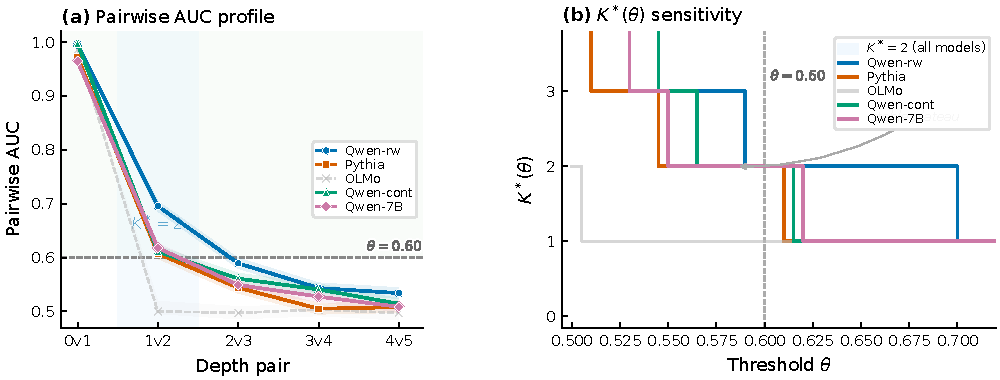
\includegraphics[width=0.75\textwidth]{figures/fig_kstar_theta.pdf}
\caption{$\Kempirical(\theta)$ sensitivity curve for five configurations. $\Kempirical$: maximum discriminable depth; $\theta$: AUC decision threshold. Four of five configurations yield $\Kempirical{=}2$ at $\theta{=}0.60$ (dashed line); OLMo yields $\Kempirical{=}1$. At $\theta{=}0.70$, all drop to $\Kempirical{=}1$.}
\label{fig:kstar_theta}
\end{figure*}

Figure~\ref{fig:kstar_theta} displays the sensitivity surface across $\theta \in [0.50, 0.70]$: four of five configurations shown yield $\Kempirical \geq 2$ for $\theta \leq 0.60$ (OLMo: $\Kempirical = 1$ throughout); at $\theta{=}0.55$, two Qwen configurations reach $\Kempirical = 3$; at $\theta{=}0.70$, all drop to $\Kempirical = 1$.
$\Kempirical{=}2$ is stable across $\theta \in [0.59, 0.60]$; at $\theta{=}0.61$, one borderline case (Pythia-1.4B) drops to $\Kempirical{=}1$.

%% ====================================================================
\subsection{Cross-Model Transfer}
\label{sec:transfer}

\begin{figure}[!t]
\centering
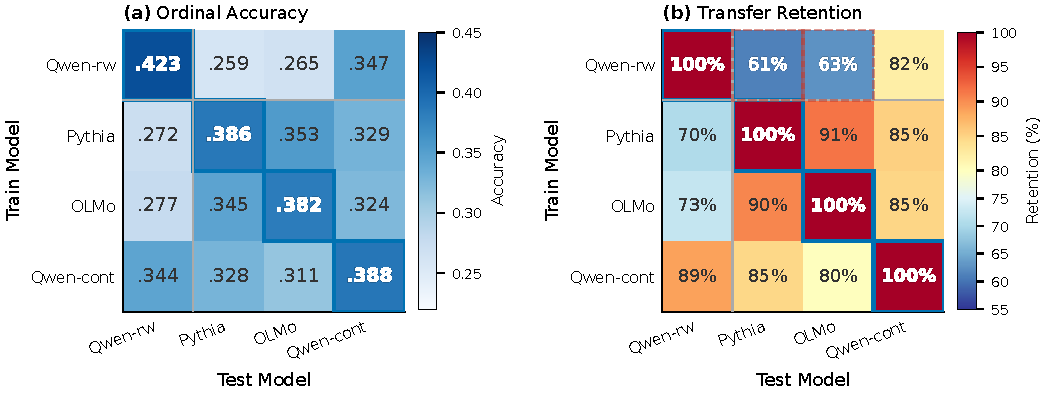
\includegraphics[width=\columnwidth]{figures/fig3_transfer_heatmap.pdf}
\vspace{-6pt}
\caption{Cross-model transfer heatmap (three continuation-mode models plus Qwen-rewrite). \textbf{(a)} 6-class ordinal accuracy when trained on the row model and evaluated on the column model; diagonal entries (highlighted) are in-domain baselines. \textbf{(b)} Retention rate (off-diagonal accuracy divided by in-domain accuracy). Continuation-mode pairs retain 80--92\%; Qwen-rw transfers at 61--63\% to other architectures but 82\% to Qwen-cont, consistent with a mode-specific artifact.}
\label{fig:transfer_heatmap}
\end{figure}

Continuation-mode classifiers transfer well across generators (Figure~\ref{fig:transfer_heatmap}; full matrix in Table~\ref{tab:s1_transfer}): Pythia$\leftrightarrow$OLMo retains 90--92\%, Qwen-cont$\leftrightarrow$Pythia 84--85\%, Qwen-cont$\leftrightarrow$OLMo 80--85\%.
Cross-scale transfer from Gemma-2-27B retains $>$100\% accuracy on 1B--8B models (101.3\% avg; ${\leq}$1.5B$\to$27B: 76.5\%); larger models may learn a universal depth-feature superset (Table~\ref{tab:gemma27b_transfer}; filtering validation in Table~\ref{tab:gemma27b_filtering}).
Qwen-rewrite classifiers transfer at 61--63\% to Pythia and OLMo but retain 82\% to Qwen-cont; cross-architecture degradation reflects a mode-specific artifact, while the within-family retention points to a Qwen-specific component layered on top.

\paragraph{Cross-scorer validation.}
Replacing the self-scorer with Pythia-1.4B or OLMo-1B preserves feature rankings ($\rho > 0.90$) but attenuates absolute discriminability at the boundary (Table~\ref{tab:crossscorer}; $\Kempirical$ comparison in Table~\ref{tab:s13_scorer_sensitivity}).
Feature ranking independence is a strong result: the same features dominate under all scorers (Table~\ref{tab:crossscorer}).
$\Kempirical$ agreement, however, is signal-strength dependent: Qwen-rewrite (strong signal, 1v2 $\auc = 0.696$) retains $\Kempirical{=}2$ under all scorers, but Qwen-continuation (marginal, 1v2 $\auc = 0.611$, only 0.011 above $\theta$) drops to $\Kempirical{=}1$ (Pythia: $0.5923$; OLMo: $0.5858$).
A three-way analysis of variance (ANOVA) (Generator $\times$ Scorer $\times$ Depth-Pair; Table~\ref{tab:anova_crossscorer}) confirms a statistically significant but modest Scorer main effect ($\eta^2_p{=}.192$, $p < .001$) and a significant Generator$\times$Scorer interaction ($\eta^2_p{=}.170$); absolute AUC values are thus scorer-dependent even when $\Kempirical$ classifications largely agree.

%% ====================================================================
\subsection{Feature Ordering and Generation Mode}
\label{sec:feature_degradation}
\label{sec:generation_mode}

Among continuation-mode models, single-feature $\auc$ rankings are highly correlated ($\rho \geq 0.85$; Table~\ref{tab:top_features}).
The top-3 features (\texttt{surp\_d1\_std}, \texttt{surp\_std}, \texttt{surp\_d2\_std}) are shared across all three families: autoregressive generation progressively damps surprisal variability.
Qwen-rewrite diverges (\texttt{freq\_entropy} dominates), consistent with its low cross-architecture transfer (61--63\% to Pythia/OLMo; 82\% within Qwen).
Within Qwen, rewrite yields 1v2 $\auc = 0.6955$ vs.\ continuation's $0.6112$ ($\Delta = +8.4$\,pp); continuation mode is therefore recommended as the canonical condition.

%% ====================================================================
\subsection{Neural Probe}
\label{sec:neural_probe}

Replacing the 15D features with frozen encoder hidden states (multilayer perceptron (MLP) probe; Table~\ref{tab:neural_probe_crossmodel}; architecture in Table~\ref{tab:s7_neural_probe}), Qwen achieves $\Kempirical^{\text{neural}} = 3$ (2v3 $\auc = 0.6159$), while Pythia remains at $\Kempirical^{\text{neural}} = 2$ ($\auc_{2v3} = 0.5963$); OLMo yields $\Kempirical^{\text{neural}} = 1$ (1v2 $\auc = 0.5054$, consistent with its 15D boundary).
We hypothesize that the Qwen-only elevation reflects self-familiarity artifacts, consistent with the poor transfer observed in Section~\ref{sec:transfer}; the 15D features yield $\Kempirical = 2$ for most families (OLMo: $\Kempirical = 1$).

\begin{table}[t]
\centering
\footnotesize
\caption{Neural probe pairwise AUC using frozen-encoder MLP. Each cell reports AUC for classifying depth $d$ vs.\ $d{+}1$ text. $\Kempirical^{\text{neural}}$: maximum depth where AUC exceeds $\theta = 0.60$.}
\label{tab:neural_probe_crossmodel}
\resizebox{\columnwidth}{!}{%
\begin{tabular}{lccc}
\toprule
\textbf{Model} & \textbf{2v3 $\auc$} & \textbf{95\% CI} & $\Kempirical^{\text{neural}}$ \\
\midrule
Qwen-1.5B  & 0.6159 & $[0.610,\,0.622]$ & 3 \\
Pythia-1.4B & 0.5963 & $[0.589,\,0.603]$ & 2 \\
OLMo-1B    & 0.5056 & $[0.497,\,0.516]$ & 1\rlap{$^\dagger$} \\
\bottomrule
\multicolumn{4}{l}{\footnotesize $^\dagger$OLMo 1v2 $\auc = 0.5054$ (below $\theta$); $\Kempirical^{\text{neural}} = 1$.}
\end{tabular}}
\end{table}

%% ====================================================================
\subsection{Cross-Domain Variation}
\label{sec:cross_domain}

The preceding experiments use C4 (general web text).
To test domain dependence, we evaluate on Wikipedia ($n{=}5{,}000$) and arXiv abstracts ($n{=}2{,}200$) across five architecture families (Table~\ref{tab:s12_domain_ablation}).
Wikipedia yields $\Kempirical{=}2$ for Qwen-1.5B (1v2 $\auc = 0.619$; Table~\ref{tab:domain_kstar}), but $\Kempirical{=}1$ for LLaMA-8B and Mistral-7B (1v2 $\auc = 0.592,\,0.558$; both below $\theta$).
Qwen-1.5B, Pythia-1.4B, LLaMA-3.1-8B, and Mistral-7B yield $\Kempirical{=}3$ for arXiv (Table~\ref{tab:domain_kstar}): 2v3 $\auc = 0.643\;[0.628,\,0.658]$, $0.655\;[0.634,\,0.662]$, $0.622\;[0.605,\,0.635]$, and $0.628$ respectively (permutation $p < 0.001$); structured academic text thus permits discrimination to greater depth independently of architecture.
OLMo-1B is the sole exception ($\Kempirical{=}1$ across all domains; cross-scorer validated, $p{=}0.510$); Mistral-7B exhibits a monotonic staircase (Wiki${=}$1, C4${=}$1, Code${=}$2, arXiv${=}$3); $\Kempirical$ is domain-determined.
The elevated signal reflects higher per-generation distributional shift (1v2 Jensen--Shannon divergence (JSD) $= 0.077$ vs.\ ${\sim}0.01$ for C4; Figure~\ref{fig:jsd_decay}), as formulaic structure amplifies deviation from domain norms; a multi-source pooled classifier confirms that the arXiv ceiling is text-intrinsic (Appendix~\ref{sec:arxiv_multi_source}).

\begin{figure}[t]
\centering
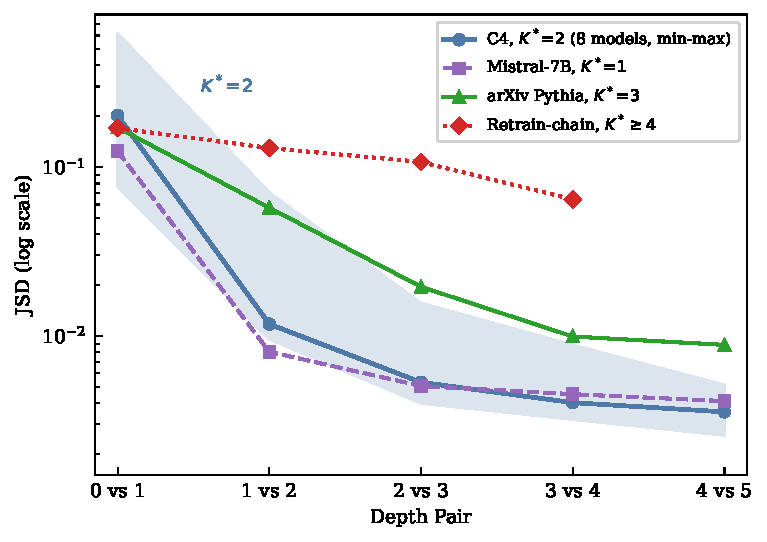
\includegraphics[width=\columnwidth]{figures/fig_jsd_decay.pdf}
\caption{JSD between adjacent depth pairs (log scale). C4 band (blue): min-max over 8 $\Kempirical{=}2$ configurations (4~model-mode pairs $+$ 4~Pythia decoding variants; $\Kempirical{=}1$ models excluded). arXiv (green) sustains signal to depth~3; retrain-chain (red) remains elevated.}
\label{fig:jsd_decay}
\end{figure}
We additionally evaluate on CodeSearchNet Python ($n{=}5{,}000$, continuation mode); all five tested models (Qwen-1.5B, Qwen-7B, LLaMA-8B, Mistral-7B, OLMo-1B) yield $\Kempirical \leq 2$ (Table~\ref{tab:domain_kstar}), matching the C4 baseline.

\begin{table}[t]
\centering
\footnotesize
\caption{Cross-domain $\Kempirical$ comparison. $\Kempirical{\leq}2$ for C4 and Code (most families $\Kempirical{=}2$; OLMo-1B: 1); $\Kempirical{=}3$ for arXiv (four families); Wikipedia varies (1--2). Mistral-7B spans all four domains, exhibiting a monotonic staircase. Bonferroni-corrected 99.5\% CI reported for the boundary pair where available (2v3 for $\Kempirical{=}3$; 1v2 otherwise).}
\label{tab:domain_kstar}
\resizebox{\columnwidth}{!}{%
\begin{tabular}{llcccc}
\toprule
\textbf{Domain} & \textbf{Model} & \textbf{1v2 $\auc$} & \textbf{2v3 $\auc$} & \textbf{Bonf CI} & $\Kempirical$ \\
\midrule
arXiv & Qwen-1.5B\rlap{$^\dagger$}  & .858 & .643 & [.628,\,.658] & 3 \\
arXiv & Pythia-1.4B & .805 & .655 & [.634,\,.662] & 3 \\
arXiv & LLaMA-8B    & .845 & .622 & [.605,\,.635] & 3 \\
arXiv & Mistral-7B  & .820 & .628 & --- & 3 \\
arXiv & OLMo-1B\rlap{$^\S$}    & .500 & .497 & [.483,\,.517] & 1 \\
C4    & Qwen-1.5B\rlap{$^\dagger$}  & .626 & .550 & --- & 2 \\
C4    & Mistral-7B  & .570 & .534 & --- & 1 \\
Code  & Qwen-1.5B\rlap{$^\dagger$}  & .738 & .530 & --- & 2 \\
Code  & Qwen-7B    & .727 & .537 & [.715,\,.739] & 2 \\
Code  & LLaMA-8B   & .739 & .511 & --- & 2 \\
Code  & Mistral-7B  & .615 & .529 & [.602,\,.628] & 2 \\
Code  & OLMo-1B\rlap{$^\S$}    & .557 & .500 & --- & 1 \\
Wiki  & Qwen-1.5B\rlap{$^\dagger$}  & .619 & .550 & --- & 2 \\
Wiki  & LLaMA-8B\rlap{$^\ddagger$}  & .592 & .538 & [.579,\,.605] & 1 \\
Wiki  & Mistral-7B  & .558 & .519 & [.543,\,.572] & 1 \\
\bottomrule
\multicolumn{6}{l}{\footnotesize $^\dagger$Qwen2.5-1.5B (base, continuation mode).} \\
\multicolumn{6}{l}{\footnotesize $^\ddagger$Marginal: point estimate $< \theta$; CI upper bound crosses 0.60.} \\
\multicolumn{6}{l}{\footnotesize $^\S$Sole exception: $K^*{=}1$ across all domains; cross-scorer validated ($p{=}0.510$, n.s.).}
\end{tabular}}
\end{table}

\paragraph{Robustness.}
\label{sec:robustness}
$\Kempirical{=}2$ holds across segment lengths of 128, 256, and 512 tokens (Table~\ref{tab:s11_length_ablation}; token-level statistics in Table~\ref{tab:token_length}); at 512 tokens the 1v2 CI lower bound falls marginally below $\theta$ but 2v3 remains well below $\theta$ at all lengths ($\leq 0.572$).
Seed robustness testing (seed $= 123$ vs.\ primary $= 42$; Table~\ref{tab:seed_robustness}) confirms $\Kempirical$ stability in 2/3 configurations; the one marginal shift (Qwen-Wikipedia $\Kempirical{=}2 \to 3$, 2v3 $\auc = 0.607$) has one of five folds below $\theta$.
The ${\pm}9$\,pp absolute AUC variation across seeds strengthens the case for threshold-based $\Kempirical$ over raw AUC comparisons.

%% ====================================================================
\subsection{Binary Detector Confidence}
\label{sec:binary_confidence}

Binary detectors (DivEye~\cite{basani2026diveye}, Binoculars~\cite{hans2024binoculars}) provide no depth signal beyond the human-vs.-machine boundary: $\Kempirical^{\text{binary}} \leq 1$, with moderate rank correlations ($|\rho| = 0.06$--$0.46$) driven entirely by the 0v1 gap (Table~\ref{tab:s9_binary_spearman}).


% === Section 5: K*-Aware Data Filtering ===
\section{Consistency Check: $\Kstar$-Guided Filtering}
\label{sec:filtering}

$\Kempirical = 2$ makes a falsifiable prediction: binary curation should suffice, and graduated performance should converge toward binary as the decay steepness increases.
We present this as a consistency check under extreme contamination, not as an independent contribution; at realistic rates ($\leq$50\%), strategy differences remain below 0.3\,pp (Appendix~\ref{sec:dose_response}).
We compare six strategies on 30{,}000 documents (depths 0--5): (i)~\textbf{no-filter}, (ii)~\textbf{binary-ours} ($w = 1 - P(\text{synthetic})$ from 15D LightGBM), (iii)~\textbf{binary-Drayson}~\citep{drayson2025}, (iv)~\textbf{graduated} ($w = \exp(-\alpha \cdot \hat{d})$, $\alpha \in \{0.1,\ldots,0.9\}$), (v)~\textbf{surprisal} (retain above median), and (vi)~\textbf{DSIR}~\citep{xie2023dsir}.
We fine-tune Qwen2.5-1.5B-Instruct via Low-Rank Adaptation (LoRA; rank~8, $\alpha_{\text{LoRA}}{=}16$) for 3 epochs on MMLU and HellaSwag across 5 seeds (${\sim}$83\% synthetic; depth~0 retains human seeds~\cite{shumailov2024collapse, dohmatob2024model}).

\begin{table}[t]
\centering
\small
\caption{Downstream task performance (MMLU, HellaSwag) under six data-filtering strategies. Binary-ours uses the 15D LightGBM depth classifier; Graduated applies exponentially decaying weights $w = \exp(-\alpha \hat{d})$. Mean $\pm$ std over 5 seeds. Full $\alpha$ sweep in Figure~\ref{fig:filtering_strategies}.}
\label{tab:tab_filtering_main}
\resizebox{\columnwidth}{!}{\begin{tabular}{lcc}
\toprule
\textbf{Strategy} & \textbf{MMLU} & \textbf{HellaSwag} \\
\midrule
Base model (no training) & 0.6018 & 0.6821 \\
\midrule
Binary-ours ($\Kstar{=}2$) & \textbf{0.5941}$\pm$0.0008 & \textbf{0.6701}$\pm$0.0006 \\
Binary-Drayson & 0.5913$\pm$0.0009 & 0.6691$\pm$0.0004 \\
Surprisal & 0.5894$\pm$0.0009 & 0.6641$\pm$0.0006 \\
Graduated ($\alpha{=}0.9$) & 0.5892$\pm$0.0008 & 0.6701$\pm$0.0007 \\
DSIR & 0.5869$\pm$0.0003 & 0.6631$\pm$0.0007 \\
No filter & 0.5865$\pm$0.0010 & 0.6638$\pm$0.0008 \\
\bottomrule
\end{tabular}
}
\end{table}

\begin{figure}[t]
\centering
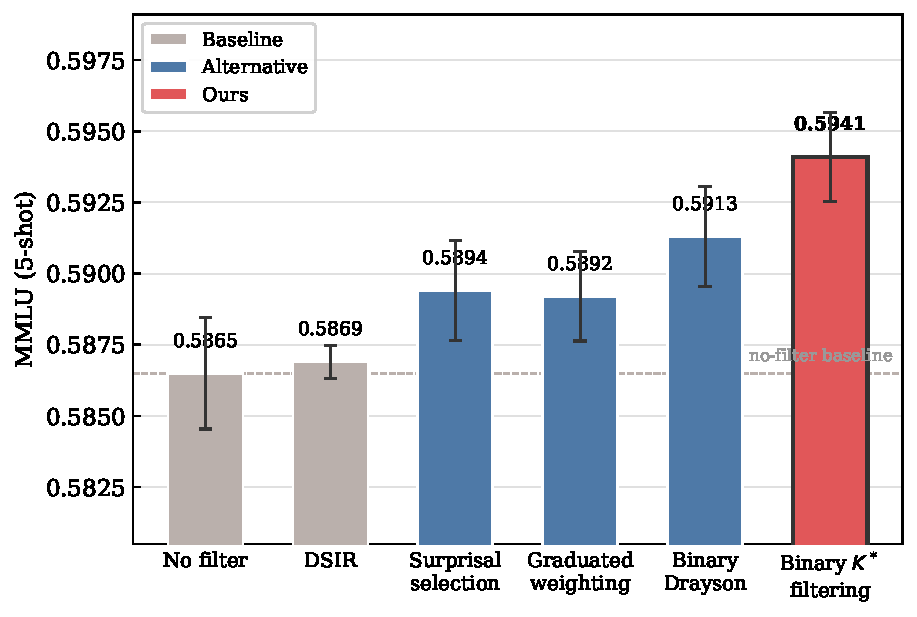
\includegraphics[width=\columnwidth]{figures/fig_filtering_strategies.pdf}
\caption{MMLU accuracy under six filtering strategies (5 seeds, $\pm$1 std). Binary $\Kstar$ filtering (red) minimizes degradation; graduated weighting converges toward binary as $\alpha$ increases. Dashed line: no-filter baseline.}
\label{fig:filtering_strategies}
\end{figure}

Binary-ours reduces the MMLU gap from $-$1.53\,pp (no-filter) to $-$0.77\,pp (${\sim}$50\% reduction; $p_{\text{corr}} < 0.05$ vs.\ all alternatives; Table~\ref{tab:tab_filtering_main}, \ref{tab:pairwise_significance}).
The ordering is interpretable through $\Kempirical$: binary filtering exploits the strongest boundary (0v1), while graduated strategies assign weights based on near-random classifier outputs, injecting noise.
Graduated filtering converges toward binary: at $\alpha{=}0.9$, it matches binary-ours on HellaSwag ($p_{\text{corr}} = 1.00$) but remains worse on MMLU ($p_{\text{corr}} = 0.011$); DSIR is indistinguishable from no-filter (Figure~\ref{fig:filtering_strategies}).
At realistic contamination ratios ($\leq$50\%), strategy differences remain below 0.3\,pp (Appendix~\ref{sec:dose_response}); this extreme setting validates $\Kempirical$'s predictive power despite vanishing effect sizes at realistic ratios.


% === Section 6: Discussion ===
\section{Discussion}
\label{sec:discussion}
\label{sec:why_kstar}
\label{sec:one_wash}
\label{sec:negative_graduated}
\label{sec:repr_dependence}
\label{sec:boundary_cases}
\label{sec:length_confound}

\paragraph{One-wash laundering (web text).}
For general web text, $\Kempirical{=}2$ reflects concentrated information loss: 0v1 is near-trivially separable ($\auc \geq 0.92$), 1v2 drops by ${\sim}$30\,pp, and 2v3 falls below $\theta$.
Converging evidence supports a data-intrinsic interpretation: OBD achieves 96\% depth-0 recall but only 14--22\% for depths $\geq$2; frontier LLMs show 8--38\% ($p > 0.05$ vs.\ OBD; Table~\ref{tab:s3_llm_zeroshot}).
Unlike model collapse~\cite{shumailov2024collapse}, one-wash laundering describes erasure of statistical fingerprints; quality may degrade further after features become indistinguishable.

\paragraph{Boundary cases and representation dependence.}
Four configurations yield $\Kempirical{=}1$; under Bonferroni correction (Table~\ref{tab:bonferroni_ci}), three of six $\Kempirical{=}2$ cases become marginal (CI lower 0.593--0.599), though the universal bound $\Kempirical \leq 2$ holds across $\theta \in [0.59, 0.61]$ (Figure~\ref{fig:kstar_theta}).
$\Kempirical$ is representation-dependent: neural probes yield $\Kempirical^{\text{neural}} \in \{1,2,3\}$ across models (Table~\ref{tab:neural_probe_crossmodel}); a DeBERTa upper-bound probe extends to $\Kempirical{=}4$ on arXiv (Table~\ref{tab:deberta_vs_obd}), placing the cost of generator-agnostic features at one depth level.

\paragraph{Domain dependence and scope.}
arXiv yields $\Kempirical{=}3$ across four families (Figure~\ref{fig:jsd_decay}), driven by larger per-generation JSD ($0.077$ vs.\ ${\sim}0.01$ for C4); markup removal preserves $\Kempirical{=}3$ ($\Delta\auc = {-}0.021$).
Retrain-chain experiments yield $\Kempirical{\geq}4$ because retraining modifies model parameters; prompt-chain $\Kempirical$ isolates text-intrinsic degradation.



% === Section 7: Conclusion ===
\section{Conclusion}
\label{sec:conclusion}

Across 10 prompt-chain configurations spanning six architecture families (1B--8B), $\Kempirical \leq 2$ for all web text sources; arXiv reaches $\Kempirical{=}3$ across four families.
One-wash laundering concentrates the exploitable signal at the 0v1 boundary: binary curation halves MMLU loss, cross-model transfer retains 80--92\% accuracy, and feature rankings remain scorer invariant ($\rho > 0.90$); graduated strategies offer no benefit beyond $\Kempirical$.
Depth-chain generation beyond 8B and closing the $\Kempirical$--$\Ktheory$ gap remain open.


% === Limitations (ACL required, unnumbered) ===
\newpage
\section*{Limitations}

(1)~\emph{Scope}: depth chains are generated by models up to 8B across 6 architecture families in English only (Gemma-2-27B is used for cross-scale transfer but not full depth-chain generation); systematic evaluation at larger scale, on RLHF/DPO-aligned models, and under retrain-chain dynamics remains open.
(2)~\emph{Features}: the 15 statistical features provide a lower bound on $\Ktheory$; richer representations can extend $\Kempirical$ by one depth level, and cross-model transfer is validated only within continuation mode.
(3)~\emph{Threshold and domain}: $\Kempirical$ varies with $\theta$ (2--3 at 0.55, 1 at 0.70; three of ten configurations are marginal at $\theta{=}0.60$), and arXiv $\Kempirical{=}3$ is established on a single structured domain.

\section*{Ethical Considerations}

This work develops tools for detecting recursive synthetic text contamination in training corpora.
The depth estimation framework is intended for dataset curation and quality auditing, not for content moderation or individual authorship attribution.
Our finding that web text becomes indistinguishable beyond two generation passes ($\Kempirical \leq 2$) has implications for data governance: it highlights a fundamental limit on provenance tracking using distributional features, which policymakers and dataset curators should consider when designing data pipelines.

\bibliography{references}

\appendix
\setlength{\floatsep}{6pt plus 2pt minus 2pt}
\setlength{\textfloatsep}{8pt plus 2pt minus 2pt}
\setlength{\intextsep}{6pt plus 2pt minus 2pt}
\setlength{\abovecaptionskip}{4pt}
\setlength{\belowcaptionskip}{2pt}
\section{Supplementary Materials}
\label{sec:appendix}

This appendix provides supplementary figures, detailed experimental tables, dataset statistics, and complete feature descriptions referenced in the main text.

\paragraph{Feature ranking and cross-model consistency.}
Table~\ref{tab:top_features} reports per-model single-feature AUC rankings.
Surprisal derivative features (\texttt{surp\_d1\_std}, \texttt{surp\_d2\_std}) consistently rank among the top three across all continuation-mode models (Pythia, OLMo, Qwen-cont), with pairwise Spearman $\rho \geq 0.85$.
The rewrite-mode model (Qwen-rw) diverges by placing \texttt{freq\_entropy} first, reflecting a distributional shift that is lexical rather than surprisal-driven.
This scorer-invariant ranking supports the use of a fixed 15-dimensional feature set across generators without per-model feature selection.

%%% Feature ranking table (moved from main text)
\begin{table}[!htbp]
\centering
\small
\caption{Top-3 features by single-feature $\auc$ ranking. Bold: shared across all continuation-mode models. Spearman $\rho$ (continuation pairs): Pythia--OLMo 0.95, Pythia--Qwen-cont 0.91, OLMo--Qwen-cont 0.85.}
\label{tab:top_features}
\resizebox{\columnwidth}{!}{%
\begin{tabular}{cllll}
\toprule
Rank & Pythia & OLMo & Qwen-rw & Qwen-cont \\
\midrule
1 & \textbf{\texttt{surp\_d1\_std}} & \textbf{\texttt{surp\_std}} & \texttt{freq\_entropy} & \textbf{\texttt{surp\_d1\_std}} \\
2 & \textbf{\texttt{surp\_d2\_std}} & \textbf{\texttt{surp\_d1\_std}} & \textbf{\texttt{surp\_std}} & \textbf{\texttt{surp\_std}} \\
3 & \textbf{\texttt{surp\_std}} & \textbf{\texttt{surp\_d2\_std}} & \textbf{\texttt{surp\_d1\_std}} & \textbf{\texttt{surp\_d2\_std}} \\
\bottomrule
\end{tabular}
}
\end{table}

Table~\ref{tab:s1_transfer} reports the cross-model transfer accuracy matrix.
Classifiers trained on continuation-mode generators (Pythia, OLMo, Qwen-cont) transfer well to each other, with off-diagonal accuracy retaining 80--92\% of in-distribution performance.
Rewrite-mode classifiers transfer at 61--63\% to other architectures but retain 82\% within Qwen, confirming that generation mode is the primary axis of distributional variation while a Qwen-specific artifact component persists (Section~\ref{sec:discussion}).

%%% Table S1: Cross-Transfer Confusion Matrix (exp-013)
\begin{table}[!htbp]
  \centering
  \small
  \caption{Cross-model transfer accuracy matrix. Diagonal (\textbf{bold}): within-model; off-diagonal: cross-model. Retention: Pythia$\leftrightarrow$OLMo 89--92\%, Qwen-cont$\leftrightarrow$Pythia 84--85\%, Qwen-rw$\to$Pythia/OLMo 61--63\%, Qwen-rw$\to$Qwen-cont 82\%.}
  \label{tab:s1_transfer}
  \resizebox{\columnwidth}{!}{%
  \begin{tabular}{lcccc}
    \toprule
    \textbf{Train} & Qwen-rw & Pythia & OLMo & Qwen-cont \\
    \midrule
    Qwen-rw   & \textbf{.423} & .259 & .265 & .347 \\
    Pythia    & .272 & \textbf{.386} & .353 & .329 \\
    OLMo      & .277 & .345 & \textbf{.382} & .324 \\
    Qwen-cont & .344 & .328 & .311 & \textbf{.388} \\
    \bottomrule
  \end{tabular}}
\end{table}

\paragraph{Dataset construction.}
Table~\ref{tab:s4_dataset_stats} summarizes the generational depth corpus.
Each depth level contains 5{,}000 passages, yielding 30{,}000 total samples across six depths (0--5).
Depth~0 consists of human-written seed texts from the C4 English validation split, truncated to 256 subword tokens.
Subsequent depths are generated recursively: each depth-$k$ passage is produced by prompting the generator with the corresponding depth-$(k{-}1)$ passage.
All six primary configurations (Qwen2.5-1.5B-Instruct rewrite and continuation, Qwen2.5-1.5B base, Qwen2.5-7B, Pythia-1.4B, OLMo-1B; Table~\ref{tab:setup}) share identical depth-0 seeds, differing only in generator model, scale, and prompting strategy.

%%% Table S4: Dataset Statistics
\begin{table}[!htbp]
  \centering
  \small
  \caption{Dataset statistics for the generational depth corpus. Depth~0 contains human-written seed texts sampled from the C4 English validation split and truncated to 256 subword tokens. Depths~1--5 are recursively generated by Qwen2.5-1.5B-Instruct (nucleus sampling, $p{=}0.95$, $T{=}1.0$). Token counts use whitespace tokenization. Statistics shown for the primary Qwen-rewrite corpus; the other five configurations share the same corpus structure.}
  \label{tab:s4_dataset_stats}
  \resizebox{\columnwidth}{!}{%
  \begin{tabular}{clrl}
    \toprule
    \textbf{Depth} & \textbf{$N$ samples} & \textbf{Mean tokens} & \textbf{Source} \\
    \midrule
    0 & 5{,}000 & 147.8 & C4 validation (human) \\
    1 & 5{,}000 & 207.1 & Qwen2.5-1.5B rewrite \\
    2 & 5{,}000 & 206.1 & Qwen2.5-1.5B rewrite \\
    3 & 5{,}000 & 208.0 & Qwen2.5-1.5B rewrite \\
    4 & 5{,}000 & 207.7 & Qwen2.5-1.5B rewrite \\
    5 & 5{,}000 & 207.7 & Qwen2.5-1.5B rewrite \\
    \midrule
    \multicolumn{2}{l}{Total} & \multicolumn{2}{l}{30{,}000 samples} \\
    \bottomrule
  \end{tabular}}
\end{table}

%%% Table S2: Decoding Ablation AUC (exp-003)
\begin{table*}[t]
  \centering
  \caption{Pairwise AUC with bootstrap 95\% CIs across depth pairs for four decoding configurations (all using Qwen2.5-1.5B-Instruct in rewrite mode; 10{,}000 bootstrap resamples). The horizontal rule between depth pairs 1\,vs.\,2 and 2\,vs.\,3 marks the empirical detectability boundary $\Kempirical=2$. Bottom rows report cross-configuration Spearman $\rho$ on per-feature discriminative-power rankings.}
  \label{tab:s2_decoding}
  \footnotesize
  \begin{tabular}{lcccc}
    \toprule
    \textbf{Depth Pair} & \textbf{Greedy} & \textbf{Nuc $p{=}0.9$, $T{=}1.0$} & \textbf{Nuc $p{=}0.95$, $T{=}0.7$} & \textbf{Nuc $p{=}0.95$, $T{=}1.2$} \\
    \midrule
    0 vs.\ 1 & $.980\;[.977,\,.982]$ & $.995\;[.993,\,.996]$ & $.988\;[.986,\,.990]$ & $.998\;[.998,\,.999]$ \\
    1 vs.\ 2 & $.689\;[.680,\,.698]$ & $.687\;[.677,\,.695]$ & $.689\;[.680,\,.697]$ & $.704\;[.695,\,.713]$ \\
    \cmidrule(lr){1-5}
    2 vs.\ 3 & $.561\;[.552,\,.571]$ & $.592\;[.582,\,.601]$\rlap{$^\dagger$} & $.590\;[.581,\,.600]$ & $.582\;[.572,\,.592]$ \\
    3 vs.\ 4 & $.540\;[.531,\,.550]$ & $.547\;[.537,\,.557]$ & $.539\;[.529,\,.549]$ & $.529\;[.519,\,.540]$ \\
    4 vs.\ 5 & $.514\;[.503,\,.524]$ & $.507\;[.496,\,.517]^{\ddagger}$ & $.535\;[.524,\,.545]$ & $.524\;[.513,\,.535]$ \\
    \midrule
    \multicolumn{5}{l}{\textbf{Cross-config feature Spearman $\rho$}} \\
    \midrule
    \multicolumn{2}{l}{Greedy vs.\ Nuc $p{=}0.9$} & 0.600 &
    \multicolumn{1}{l}{Nuc $p{=}0.9$ vs.\ $T{=}0.7$} & 0.782 \\
    \multicolumn{2}{l}{Greedy vs.\ $T{=}0.7$} & 0.914 &
    \multicolumn{1}{l}{Nuc $p{=}0.9$ vs.\ $T{=}1.2$} & 0.893 \\
    \multicolumn{2}{l}{Greedy vs.\ $T{=}1.2$} & 0.532 &
    \multicolumn{1}{l}{$T{=}0.7$ vs.\ $T{=}1.2$} & 0.668 \\
    \bottomrule
    \multicolumn{5}{l}{${}^{\dagger}$\,CI upper bound (0.601) marginally exceeds $\theta{=}0.60$ by 0.001.} \\
    \multicolumn{5}{l}{${}^{\ddagger}$\,Permutation $p = 0.12$ (not significant). All other pairs $p < 0.01$.}
  \end{tabular}
\end{table*}

%%% Table S2b: Extended K* CI (all models including new additions)
\begin{table*}[t]
  \centering
  \footnotesize
  \caption{Extended pairwise $\auc$ with bootstrap 95\% CIs for all model configurations including new additions.
  This table extends Table~\ref{tab:kstar_ci} in the main text with Qwen-base, LLaMA-8B, Mistral-7B, Pythia-6.9B (nucleus), and Gemma-2-2B configurations.
  $\Kempirical = 2$ holds for 6/10 conditions at $\theta{=}0.60$ (OLMo-1B, Mistral-7B, Pythia-6.9B, Gemma-2-2B: $\Kempirical{=}1$).
  95\% bootstrap CIs shown in brackets where available.}
  \label{tab:kstar_ci_extended}
  \setlength{\tabcolsep}{3.5pt}
  \resizebox{\textwidth}{!}{%
  \begin{tabular}{lcccccccccc}
    \toprule
     & Qwen-rw & Pythia & OLMo & Qwen-cont & Qwen-7B$^\ddagger$ & Qwen-base & LLaMA-8B & Mistral-7B & Pythia-6.9B$^\S$ & Gemma-2B \\
    \midrule
    0v1 & .9956 & .9722 & .9860 & .9971 & .9644\,[.961,.967] & .987\,[.985,.989] & .9224\,[.917,.927] & .9209\,[.919,.923] & .9599 & .953\,[.949,.957] \\
    1v2 & \textbf{.6955}\,[.686,.704]$^*$ & \textbf{.6074}\,[.598,.617]$^*$ & .5001\,[.496,.519] & \textbf{.6112}\,[.602,.621]$^*$ & \textbf{.6178}\,[.608,.626]$^*$ & \textbf{.626}\,[.617,.635]$^*$ & \textbf{.6123}\,[.603,.622]$^*$ & .5695\,[.565,.575] & .5955 & .5981\,[.588,.608] \\
    2v3 & .5893\,[.580,.599] & .5440\,[.534,.554] & .4973\,[.486,.509] & .5609\,[.551,.571] & .5492\,[.539,.559] & .550\,[.540,.560] & .5273\,[.517,.538] & .5335\,[.528,.538] & .5298 & .534\,[.523,.545] \\
    3v4 & .5435 & .5051 & .5034 & .5409 & .5276 & .529\,[.519,.540] & .5168\,[.506,.528] & .5140 & .5135 & .5033\,[.492,.514] \\
    4v5 & .5340 & .5079 & .4971 & .5141 & .5085 & .518\,[.508,.529] & .5159\,[.505,.527] & .5184 & ---$^\|$ & .5025\,[.492,.514] \\
    \bottomrule
    \multicolumn{11}{l}{\scriptsize $^*$Permutation $p < 0.001$ for all boundary comparisons. Bold: $\auc > \theta{=}0.60$.} \\
    \multicolumn{11}{l}{\scriptsize $^\ddagger$Generator: Qwen2.5-7B (fp16); scorer: Qwen2.5-1.5B.} \\
    \multicolumn{11}{l}{\scriptsize $^\|$$\Kempirical{=}1$; 4v5 not required for boundary determination.} \\
    \multicolumn{11}{l}{\scriptsize $^\S$Pythia-6.9B evaluated separately; nucleus sampling ($p{=}0.95$, $T{=}1.0$), same as all other models.}
  \end{tabular}}% end resizebox
\end{table*}

%%% Table S3: LLM Zero-Shot Confusion Matrices (exp-011)
\begin{table}[t]
  \centering
  \scriptsize
  \caption{LLM zero-shot depth classification: $5{\times}5$ confusion matrices (Exp-011). Both frontier LLMs achieve high binary detection accuracy (GPT-5.5: 0.878; Claude Opus~4.6: 0.882) but near-chance 5-class accuracy (${\sim}$0.33 vs.\ OBD-LightGBM 0.386). Per-depth recall in Table~\ref{tab:s3c_perdepth}.}
  \label{tab:s3_llm_zeroshot}

  \vspace{0.3em}
  \textbf{(a)} GPT-5.5 ($N{=}500$, acc${=}0.332$, MAE${=}1.102$)
  \vspace{1pt}

  \begin{tabular}{lcccccc}
    \toprule
    & \multicolumn{5}{c}{Predicted Depth} & \\
    \cmidrule(lr){2-6}
    True & 0 & 1 & 2 & 3 & 4 & Rec. \\
    \midrule
    0 & \textbf{77} & 18 &  4 &  0 &  1 & .770 \\
    1 &  9 & \textbf{19} & 36 & 24 & 12 & .190 \\
    2 &  8 & 10 & \textbf{38} & 35 &  9 & .380 \\
    3 & 10 & 16 & 35 & \textbf{24} & 15 & .240 \\
    4 & 11 & 13 & 50 & 18 &  \textbf{8} & .080 \\
    \bottomrule
  \end{tabular}

  \vspace{4pt}
  \textbf{(b)} Claude Opus~4.6 ($N{=}499$, acc${=}0.331$, MAE${=}1.150$)
  \vspace{1pt}

  \begin{tabular}{lcccccc}
    \toprule
    & \multicolumn{5}{c}{Predicted Depth} & \\
    \cmidrule(lr){2-6}
    True & 0 & 1 & 2 & 3 & 4 & Rec. \\
    \midrule
    0 & \textbf{69} & 26 &  3 &  0 &  2 & .690 \\
    1 &  8 & \textbf{21} & 32 & 11 & 28 & .210 \\
    2 &  6 & 36 & \textbf{28} &  5 & 25 & .280 \\
    3 &  7 & 20 & 31 & \textbf{10} & 31 & .100 \\
    4 &  7 & 28 & 22 &  6 & \textbf{37} & .370 \\
    \bottomrule
  \end{tabular}
\end{table}

\begin{table}[t]
  \centering
  \small
  \caption{Per-depth recall (\%) on balanced $N{=}500$ test set. OBD's nominal overall accuracy gap originates from depth-0; all methods fail at depths $\geq 2$, consistent with $\Kempirical = 2$.}
  \label{tab:s3c_perdepth}
  \resizebox{\columnwidth}{!}{%
  \begin{tabular}{lccccc}
    \toprule
    & Depth 0 & Depth 1 & Depth 2 & Depth 3 & Depth 4 \\
    \midrule
    OBD-LightGBM & \textbf{96} & \textbf{39} & 14 & 19 & 22 \\
    GPT-5.5      & 77 & 19 & \textbf{38} & \textbf{24} &  8 \\
    Claude Opus~4.6 & 69 & 21 & 28 & 10 & \textbf{37} \\
    \bottomrule
  \end{tabular}}
\end{table}

%%% Table: Token Length and EOS Truncation Analysis
\begin{table}[t]
  \centering
  \scriptsize
  \caption{Mean subword token count per depth and EOS truncation rate (\%) for depth~1+ across all model configurations (generation limit: 256 tokens). Depth~0 (human text) is shared across configurations. Depths 1--5 show no systematic length trend; the 0v1 length asymmetry (human texts shorter) makes detection \emph{more conservative}, not inflated. See Section~\ref{sec:length_confound}.}
  \label{tab:token_length}
  \resizebox{\columnwidth}{!}{%
  \begin{tabular}{lcccccccc}
    \toprule
    & \multicolumn{6}{c}{\textbf{Mean Token Count}} & & \\
    \cmidrule(lr){2-7}
    \textbf{Model} & D0 & D1 & D2 & D3 & D4 & D5 & \textbf{EOS\%} & \textbf{Sev.} \\
    \midrule
    Qwen-rw (1.5B)  & 191 & 254 & 252 & 254 & 254 & 254 & 7--11 & Mild \\
    Pythia-1.4B      & 192 & 214 & 215 & 216 & 217 & 218 & 34--36 & High \\
    OLMo-1B          & 192 & 256 & 256 & 256 & 256 & 256 & $<$1 & Negl. \\
    Qwen-cont (1.5B) & 191 & 244 & 238 & 240 & 240 & 238 & 17--20 & Mod. \\
    Qwen-7B          & 191 & 196 & 195 & 193 & 197 & 197 & 45--47 & High \\
    \midrule
    \multicolumn{9}{l}{\textit{Decoding ablation (Qwen-rw 1.5B)}} \\
    \quad Greedy          & 191 & 253 & 252 & 253 & 254 & 254 & 8--12 & Mild \\
    \quad Nuc $p{=}0.9$   & 191 & 254 & 251 & 254 & 253 & 254 & 8--16 & Mild \\
    \quad $T{=}0.7$       & 191 & 253 & 251 & 253 & 253 & 254 & 8--14 & Mild \\
    \quad $T{=}1.2$       & 191 & 254 & 252 & 253 & 254 & 254 & 8--16 & Mild \\
    \bottomrule
    \multicolumn{9}{l}{EOS\%: generation terminated via EOS before 256-token limit. Ranges span depths 1--5.}
  \end{tabular}}
\end{table}

%%% Table S5: Complete 15-D Feature Descriptions
\begin{table*}[t]
  \centering
  \caption{Complete description of the 15-dimensional feature set used by the OBD classifier. Features are grouped into four groups: surprisal moments (4~dims) and surprisal derivatives (5~dims) computed from Qwen2.5-1.5B token-level log-probabilities, lexical diversity (3~dims), and frequency tail shape (3~dims). All features are computed per document.}
  \label{tab:s5_features}
  \begin{tabular}{llp{0.45\textwidth}l}
    \toprule
    \textbf{Group} & \textbf{Feature} & \textbf{Description} & \textbf{Range} \\
    \midrule
    \multirow{9}{*}{\rotatebox[origin=c]{90}{\textsc{Surprisal}}}
    & \texttt{surp\_mean}   & Mean token surprisal $\frac{1}{T}\sum_t -\log p(x_t \mid x_{<t})$ & $\mathbb{R}^+$ \\
    & \texttt{surp\_std}    & Standard deviation of token surprisal & $\mathbb{R}^+$ \\
    & \texttt{surp\_skew}   & Skewness of the surprisal distribution & $\mathbb{R}$ \\
    & \texttt{surp\_kurt}   & Excess kurtosis of the surprisal distribution & $\mathbb{R}$ \\
    & \texttt{surp\_d1\_mean} & Mean of first-order surprisal differences $\Delta s_t = s_{t+1} - s_t$ & $\mathbb{R}$ \\
    & \texttt{surp\_d1\_std}  & Std of first-order surprisal differences & $\mathbb{R}^+$ \\
    & \texttt{surp\_d1\_skew} & Skewness of first-order surprisal differences & $\mathbb{R}$ \\
    & \texttt{surp\_d2\_mean} & Mean of second-order differences $\Delta^2 s_t$ & $\mathbb{R}$ \\
    & \texttt{surp\_d2\_std}  & Std of second-order surprisal differences & $\mathbb{R}^+$ \\
    \midrule
    \multirow{3}{*}{\rotatebox[origin=c]{90}{\textsc{Lex}}}
    & \texttt{ttr}          & Type-token ratio: $|V| / T$ & $[0, 1]$ \\
    & \texttt{hapax\_ratio} & Hapax legomena ratio: freq-1 types / unique types & $[0, 1]$ \\
    & \texttt{self\_bleu}   & Mean 4-gram BLEU against 100 random same-depth samples & $[0, 1]$ \\
    \midrule
    \multirow{3}{*}{\rotatebox[origin=c]{90}{\textsc{Freq}}}
    & \texttt{freq\_kurtosis}  & Excess kurtosis of word frequency distribution & $\mathbb{R}$ \\
    & \texttt{freq\_entropy}   & Shannon entropy of word frequencies: $-\sum p_w \log_2 p_w$ & $\mathbb{R}^+$ \\
    & \texttt{low\_freq\_ratio} & Proportion of vocabulary with count $\leq 2$ & $[0, 1]$ \\
    \bottomrule
  \end{tabular}
\end{table*}

%%% Tables S6 & S7: Side by side in a single table* to avoid table*/table overlap
\begin{table*}[t]
\begin{minipage}[t]{0.45\textwidth}
  \centering
  \small
  \captionof{table}{LightGBM hyperparameters for the OBD (Ordinal Binary Decomposition) classifier used throughout the paper. One cumulative binary classifier is trained for each threshold $k$, predicting whether depth $> k$. Pairwise AUCs are derived from adjacent-depth comparisons to evaluate separability. 5-fold GroupKFold cross-validation is grouped by \texttt{doc\_id} to prevent data leakage from the same seed document appearing in both train and test.}
  \label{tab:s6_lgbm_params}
  \begin{tabular}{ll}
    \toprule
    \textbf{Parameter} & \textbf{Value} \\
    \midrule
    \texttt{n\_estimators}      & 200 \\
    \texttt{learning\_rate}     & 0.05 \\
    \texttt{max\_depth}         & 6 \\
    \texttt{num\_leaves}        & 31 \\
    \texttt{verbose}            & $-1$ \\
    \texttt{n\_jobs}            & $-1$ (all cores) \\
    Cross-validation            & 5-fold GroupKFold \\
    Grouping key                & \texttt{doc\_id} \\
    Objective                   & Binary (per depth pair) \\
    \bottomrule
  \end{tabular}
\end{minipage}\hfill
\begin{minipage}[t]{0.52\textwidth}
  \centering
  \small
  \captionof{table}{Neural probe architecture and training details (Exp-015). Applied to all three model families (Qwen2.5-1.5B, Pythia-1.4B, OLMo-1B): each model's frozen hidden states are average-pooled into document embeddings and classified by a two-hidden-layer MLP.}
  \label{tab:s7_neural_probe}
  \resizebox{\textwidth}{!}{%
  \begin{tabular}{ll}
    \toprule
    \textbf{Component} & \textbf{Details} \\
    \midrule
    \multicolumn{2}{l}{\textit{Embedding extraction}} \\
    Base models       & Qwen2.5-1.5B / Pythia-1.4B / OLMo-1B (frozen) \\
    Representation    & Last hidden state, attention-masked avg pool \\
    Embedding dim     & 1536 / 2048 / 2048 \\
    Max sequence len   & 512 tokens \\
    \midrule
    \multicolumn{2}{l}{\textit{MLP classifier}} \\
    Architecture      & $d_{\text{emb}} \to 512 \to 256 \to 6$ \\
    Activations       & ReLU \\
    Dropout           & 0.1 (after each hidden layer) \\
    Output            & 6-class softmax \\
    \midrule
    \multicolumn{2}{l}{\textit{Training}} \\
    Optimizer         & Adam ($\text{lr} = 10^{-3}$, weight decay $= 10^{-4}$) \\
    Loss              & Cross-entropy \\
    Batch size        & 256 \\
    Max epochs        & 20 \\
    Early stopping    & Patience = 5 (validation loss) \\
    Cross-validation  & 5-fold GroupKFold \\
    \bottomrule
  \end{tabular}%
  }
\end{minipage}
\end{table*}

%%% Table S8: Per-Model Bootstrap CI Results (exp-007)
\begin{table}[t]
  \centering
  \scriptsize
  \caption{Pairwise AUC with bootstrap 95\% CIs for four of six primary configurations (1{,}000 resamples). All boundary pairs ($\auc > \theta$) $p < 0.01$; OLMo 1v2--4v5 non-significant ($p > 0.09$).}
  \label{tab:s8_cv_folds}
  \resizebox{\columnwidth}{!}{%
  \begin{tabular}{lcccc}
    \toprule
    & \textbf{Qwen-rw} & \textbf{Pythia} & \textbf{OLMo} & \textbf{Qwen-cont} \\
    \midrule
    0v1 & $.996\;[.995,.997]$ & $.972$ & $.986\;[.984,.988]$ & $.997\;[.996,.998]$ \\
    1v2 & $.696\;[.686,.704]$ & $.607\;[.598,.617]$ & $.500\;[.496,.519]$ & $.611\;[.602,.621]$ \\
    \cmidrule(lr){1-5}
    2v3 & $.589\;[.580,.599]$ & $.544\;[.534,.554]$ & $.497\;[.486,.509]$ & $.561\;[.551,.571]$ \\
    3v4 & $.544\;[.533,.555]$ & $.505$ & $.503\;[.491,.513]$ & $.541\;[.531,.551]$ \\
    4v5 & $.534\;[.524,.545]$ & $.508$ & $.497\;[.483,.506]$ & $.514\;[.504,.526]$ \\
    \bottomrule
  \end{tabular}}
\end{table}

%%% Table S9: Binary Detector Spearman ρ (exp-012)
\begin{table}[t]
  \centering
  \scriptsize
  \caption{Spearman $\rho$ between binary detector scores and true depth, and 6-class accuracy. Correlations driven by 0v1; scores do not track depth beyond generation~1. Qwen-rw exhibits reversed sign ($\rho > 0$).}
  \label{tab:s9_binary_spearman}
  \resizebox{\columnwidth}{!}{%
  \begin{tabular}{lcccc}
    \toprule
    & \textbf{Qwen-rw} & \textbf{Pythia} & \textbf{OLMo} & \textbf{Qwen-cont} \\
    \midrule
    \multicolumn{5}{l}{\textit{Spearman $\rho$}} \\
    \quad log-PPL (ref)      & $-0.123$ & $-0.297$ & $-0.378$ & $-0.389$ \\
    \quad log-PPL (obs.)     & $+0.082$ & $-0.453$ & $-0.461$ & $-0.162$ \\
    \quad PPL ratio           & $+0.119$ & $-0.392$ & $-0.407$ & $-0.058$ \\
    \midrule
    6-class acc.              & 0.199    & 0.130    & 0.127    & 0.183 \\
    \bottomrule
    \multicolumn{5}{l}{Random baseline: 0.167} \\
  \end{tabular}}
\end{table}

%%% Table S10: Pythia Decoding Ablation (exp-020)
\begin{table}[t]
  \centering
  \scriptsize
  \caption{Pythia-1.4B pairwise $\auc$ under four decoding configs (10K bootstrap). $^\dagger$Greedy triggers repetition collapse (4-gram repeat: $d_0{=}0.01 \to d_1{=}0.72$).}
  \label{tab:s10_pythia_decoding}
  \resizebox{\columnwidth}{!}{%
  \begin{tabular}{lcccc}
    \toprule
    & \textbf{Greedy}$^\dagger$ & \textbf{$p{=}0.9$} & \textbf{$T{=}0.7$} & \textbf{$T{=}1.2$} \\
    \midrule
    0v1 & $.999$ & $.995$ & $.997$ & $.993$ \\
    1v2 & $.884$ & $.677$ & $.727$ & $.617$ \\
    \cmidrule(lr){1-5}
    2v3 & $.534$ & $.555$ & $.594^\ddagger$ & $.523$ \\
    3v4 & $.523$ & $.530$ & $.570$ & $.517$ \\
    4v5 & $.516$ & $.501$ & $.528$ & $.505$ \\
    \midrule
    $\Kempirical$ & 2 & 2 & 2 & 2 \\
    \bottomrule
    \multicolumn{5}{l}{${}^{\ddagger}$CI upper 0.606 $> \theta$; point est.\ below.} \\
  \end{tabular}}
\end{table}

%%% Table S11: Length Ablation (exp-021)
\begin{table}[t]
  \centering
  \small
  \caption{Pairwise $\auc$ for three segment lengths (Qwen-base, cont.\ mode). $\Kempirical{=}2$ at 128/256; 512 marginal ($^\dagger$CI lower $< \theta$).}
  \label{tab:s11_length_ablation}
  \begin{tabular}{lccc}
    \toprule
    & \textbf{128} & \textbf{256} & \textbf{512} \\
    \midrule
    0v1 & .979 & .991 & .992 \\
    1v2 & .622 & .628 & .607$^\dagger$ \\
    \cmidrule(lr){1-4}
    2v3 & .529 & .556 & .572 \\
    3v4 & .535 & .530 & .530 \\
    4v5 & .501 & .514 & .518 \\
    \midrule
    $\Kempirical$ & 2 & 2 & 2$^\dagger$ \\
    \bottomrule
  \end{tabular}
\end{table}

%%% Table S12: Domain Ablation
\begin{table}[t]
  \centering
  \small
  \caption{Pairwise $\auc$ for three text domains (Qwen-cont). arXiv yields $\Kempirical{=}3$; C4 and Wikipedia $\Kempirical{=}2$.}
  \label{tab:s12_domain_ablation}
  \begin{tabular}{lccc}
    \toprule
    & \textbf{C4} & \textbf{Wiki} & \textbf{arXiv} \\
    \midrule
    0v1 & .997 & .996 & .995 \\
    1v2 & .611 & .619 & .858 \\
    \cmidrule(lr){1-4}
    2v3 & .561 & .550 & .643$^*$ \\
    3v4 & .541 & .523 & .544 \\
    4v5 & .514 & .514 & .529 \\
    \midrule
    $\Kempirical$ & 2 & 2 & 3 \\
    \bottomrule
    \multicolumn{4}{l}{\footnotesize $^*$CI $[.628,.658]$; $p < 0.001$.}
  \end{tabular}
\end{table}

%%% Table S13: Scorer Sensitivity Analysis
\begin{table}[t]
  \centering
  \scriptsize
  \caption{Scorer sensitivity: $\Kempirical$ under self- vs.\ cross-scoring. Cross-scoring reduces $\Kempirical$ only for marginal Qwen-cont.}
  \label{tab:s13_scorer_sensitivity}
  \resizebox{\columnwidth}{!}{%
  \begin{tabular}{llcccc}
    \toprule
    \textbf{Generator} & \textbf{Mode} & \textbf{Self} & \textbf{Pythia} & \textbf{OLMo} & \textbf{Agr.} \\
    \midrule
    Qwen-Inst & Rewrite & 2 & 2 & 2 & \checkmark \\
    Qwen-Inst & Cont.   & 2 & 1 & 1 & $\times$ \\
    Qwen-base & Cont.   & 2 & 2 & 2 & \checkmark \\
    Pythia    & Cont.   & 2 & 2 & 2 & \checkmark \\
    OLMo      & Cont.   & 1 & -- & -- & -- \\
    Qwen-7B   & Cont.   & 2 & -- & -- & -- \\
    Mistral   & Cont.   & 1 & -- & -- & -- \\
    \bottomrule
  \end{tabular}}
\end{table}

\clearpage

\section{Extended Discussion}
\label{sec:extended_discussion}

\subsection{Theoretical Implications of $\Kempirical = 2$}

The DPI guarantees a finite $\Ktheory$; for general web text, $\Kempirical \leq 2$ across all 10 configurations (1B--8B, 6 families), while structured domains (arXiv) yield $\Kempirical{=}3$, aligning with model collapse convergence~\cite{shumailov2024collapse, dohmatob2024model, alemohammad2024selfconsuming}.
Decoding strategy modestly affects signal strength (1v2 $\auc \in [0.6862, 0.7037]$) but does not shift the boundary.

\subsection{Cross-Model Transfer Implications}

Cross-model classification retains 80--92\% accuracy with scorer-invariant feature rankings ($\rho > 0.90$), enabling single-classifier deployment across generators.
Absolute discriminability at the $\Kempirical$ boundary is scorer-sensitive: alternative scorers reduce Qwen-continuation $\Kempirical$ from 2 to 1, while rewrite-mode $\Kempirical = 2$ is preserved.
Model family similarity modulates transfer (Pythia$\leftrightarrow$OLMo: 89--92\% vs.\ Qwen-cont$\leftrightarrow$OLMo: 80--85\%).

\begin{minipage}{\columnwidth}
\centering
\captionof{table}{Cross-scorer validation. Alternative scorers (Pythia-1.4B, OLMo-1B) preserve feature ranking ($\rho > 0.90$) and rewrite-mode $\Kempirical = 2$, but reduce continuation-mode $\Kempirical$ from 2 to 1. OLMo arXiv cross-scorer confirms $\Kempirical{=}1$ ($p{=}0.510$, n.s.).}
\label{tab:crossscorer}
\resizebox{\columnwidth}{!}{{\small
\begin{tabular}{llcccc}
\toprule
\textbf{Scorer} & \textbf{Gen.\ Data} & $\boldsymbol{K^*}$ & \textbf{AUC(0v1)} & \textbf{AUC(1v2)} & \textbf{Spearman}~$\boldsymbol{\rho}$ \\
\midrule
% --- Qwen-RW block ---
Qwen-1.5B (self) & Qwen-RW & 2 & --- & 0.6955 & --- \\
Pythia-1.4B       & Qwen-RW & 2 & 0.9923 & 0.7012 & 0.906 \\
OLMo-1B           & Qwen-RW & 2 & 0.9918 & 0.6947 & 0.920 \\
\midrule
% --- Qwen-cont block ---
Qwen-1.5B (self) & Qwen-cont & 2 & --- & 0.6112 & --- \\
Pythia-1.4B       & Qwen-cont & \textcolor{red}{1\textsuperscript{$\dagger$}} & 0.9900 & \underline{0.5923} & 0.942 \\
OLMo-1B           & Qwen-cont & \textcolor{red}{1\textsuperscript{$\dagger$}} & 0.9890 & \underline{0.5858} & 0.902 \\
\midrule
% --- Qwen-7B cross-scale block ---
Qwen-1.5B        & Qwen-7B-cont & 2 & 0.9644 & 0.6178 & --- \\
\midrule
% --- OLMo cross-scorer block (all domains) ---
Cross-scorer      & OLMo-arXiv   & 1 & 0.999  & 0.500\textsuperscript{n.s.} & --- \\
Cross-scorer      & OLMo-Code    & 1 & 0.9996 & 0.557\textsuperscript{n.s.} & --- \\
\bottomrule
\end{tabular}
}
}
\end{minipage}

\begin{table}[h]
\centering
\small
\caption{Three-way ANOVA (Generator $\times$ Scorer $\times$ Depth-Pair) on per-fold pairwise $\auc$ values. DV = per-fold AUC; $N{=}300$ (12 cells $\times$ 5 folds $\times$ 5 depth-pairs). Scorer is statistically significant but explains modest variance ($\eta^2_p{=}.192$) relative to Depth-Pair ($\eta^2_p{=}.998$), supporting near-scorer-independence of depth discrimination.}
\label{tab:anova_crossscorer}
\begin{tabular}{lrrrr}
\toprule
\textbf{Source} & \textbf{df} & $F$ & $p$ & $\eta^2_p$ \\
\midrule
Generator     & 2  & 926.78  & ${<}.001$  & .885 \\
Scorer        & 3  & 19.02  & ${<}.001$  & .192 \\
Depth-Pair    & 4  & 24736.10  & ${<}.001$  & .998 \\
Gen$\times$Scorer & 6 & 8.16 & ${<}.001$ & .170 \\
Gen$\times$Depth  & 8 & 993.69 & ${<}.001$ & .971 \\
Scorer$\times$Depth & 12 & 2.45 & $.005$ & .109 \\
Residual      & 240 & & & \\
\bottomrule
\end{tabular}
\end{table}

\subsection{Feature Importance Across Decoding Strategies}

Feature importance ordering varies across decoding strategies: greedy and $T{=}0.7$ share highly correlated rankings ($\rho = 0.914$), while greedy vs.\ $T{=}1.2$ yields lower correlation ($\rho = 0.53$, nonsignificant after Bonferroni).
The depth boundary is robust but the optimal feature subset is strategy-dependent.

\subsection{Scale and Neural Probe}
\label{sec:extended_neural_probe}

Cross-scale validation confirms $\Kempirical = 2$ from 1.5B through 8B: Qwen-7B (1v2 $\auc = 0.6178$ $[0.608, 0.626]$) and LLaMA-3.1-8B (1v2 $\auc = 0.6123$, 0v1 $= 0.9224$) both exceed $\theta$, with progressively lower 0v1 signal consistent with larger models generating more human-like text.
Gemma-2-27B (C4 continuation, Qwen cross-scored) yields $\Kempirical{=}1$ (1v2 $\auc = 0.5894$), consistent with Gemma-2-2B at 5K ($\Kempirical{=}1$, 1v2 $\auc = 0.5981$). The Gemma family produces $\Kempirical{=}1$ at both 2B and 27B, suggesting $\Kempirical$ is model-family-dependent rather than scale-dependent.

The neural probe yields model-dependent $\Kempirical^{\text{neural}}$: $3$ for Qwen (self-familiarity effect from instruction-tuned representations) but $2$ for Pythia; OLMo yields $\Kempirical^{\text{neural}} = 1$ (1v2 $\auc = 0.5054$), consistent with the 15D LightGBM boundary.
The 15D generator-agnostic features yield $\Kempirical = 2$ for Pythia and Qwen, while OLMo yields $\Kempirical = 1$ under the standardized pipeline.

\subsection{LLM Zero-Shot Baseline}
\label{sec:extended_llm}

GPT-5.5 achieves 33.2\% accuracy (MAE = 1.10) and Claude Opus~4.6 33.1\% (MAE = 1.15) on a balanced 500-sample test set, comparable to OBD-LightGBM's 38.6\% (95\% CI: $[0.340, 0.422]$; McNemar $p = 0.081$, $0.069$; Table~\ref{tab:s3_llm_zeroshot}).
Per-depth recall confirms convergent failure at depths $\geq 2$ (Section~\ref{sec:why_kstar}).
The LLM baseline evaluates depths 0--4 (5-class; Table~\ref{tab:s3_llm_zeroshot}). When probabilities are marginalized to 4 classes ($P(d{\geq}3)$), accuracy rises to 44.4\% but concentrates in the merged class while depths 2--3 collapse to 2--8\%.

\subsection{Practical Considerations}

All filtering strategies degrade general capabilities (MMLU: 0.6018 $\to$ 0.5865--0.5941; HellaSwag: 0.6821 $\to$ 0.6631--0.6701); our depth-chain setting (${\sim}$83\% synthetic) is an upper bound; in mixed corpora, degradation scales with contamination fraction~\cite{shumailov2024collapse, dohmatob2024model}.
$\Kstar$-aware binary filtering reduces MMLU degradation by ${\sim}$50\% ($-$1.53\,pp $\to$ $-$0.77\,pp), requires no per-model calibration, and is combinable with distribution-matching methods (DSIR, DoReMi).

\subsection{Additional Scope Analysis}
\label{sec:extended_limitations}

\emph{Prompt-chain versus retrain-chain.}
Retrain-chain validation (Pythia-1.4B LoRA, 5 generations) yields $\Kempirical{\geq}4$ (1v2 $\auc = 0.9484$, 2v3 $= 0.8888$, 3v4 $= 0.7982$), far exceeding prompt-chain $\Kempirical{=}2$.
The elevated signal arises from cumulative model-adaptation artifacts rather than text-intrinsic degradation; prompt-chain $\Kempirical$ is the operationally relevant boundary for data curation.

\emph{Threshold sensitivity.}
At $\theta = 0.55$, $\Kempirical = 3$ for Qwen-rewrite/continuation; at $\theta = 0.70$, $\Kempirical = 1$ across all configurations (Figure~\ref{fig:kstar_theta}).
Qwen-continuation's 1v2 CI lower bound exceeds $\theta$ by only 0.2\,pp; all ten boundary comparisons yield permutation $p < 0.001$.

\emph{Structural confound: token length.}
In continuation mode the generation prompt is discarded, so all depths $\geq 1$ consist entirely of machine-generated tokens and the 1v2 boundary compares texts differing only in conditioning context (human-authored vs.\ machine-generated prompt), not structural composition.
Depth~0 texts average ${\sim}$191 subword tokens (C4 truncation), while depth~1+ texts average 193--256 tokens depending on model (Table~\ref{tab:token_length}).
This asymmetry is directionally opposite to a length-inflation confound: shorter depth-0 texts provide less feature-extraction context, making 0v1 discrimination harder, not easier.
Within depths 1--5, mean token counts are stable (within-model range $\leq$ 4 tokens for all configurations except Qwen-continuation at 6 tokens), so the pairwise comparisons underlying $\Kempirical{=}2$ are unaffected by length.
EOS truncation rates are similarly depth-stable within each model: Qwen-rewrite 7--11\%, Pythia 34--36\%, OLMo $<$1\%, Qwen-continuation 17--20\%, Qwen-7B 45--47\%.
Models with the highest truncation (Pythia, Qwen-7B) still yield $\Kempirical{=}2$ with the same step-function AUC decay pattern as low-truncation models (Table~\ref{tab:kstar_ci}), confirming that EOS truncation does not drive the boundary.

\emph{Graduated filtering.}
All $\alpha$ values (0.1--0.9) underperform binary-ours on MMLU ($\alpha{=}0.1$: 0.5873; $\alpha{=}0.9$: 0.5892 vs.\ 0.5941); at $\alpha{=}0.9$, HellaSwag matches exactly (0.6701).
Binary-ours significantly outperforms all alternatives on MMLU ($p_{\text{corr}} \leq 0.021$); Graduated$_{0.9}$ is indistinguishable on HellaSwag ($p = 1.00$) but worse on MMLU ($p_{\text{corr}} = 0.011$).
\label{tab:pairwise_significance}

\subsection{Dose-Response: Contamination Ratio Effect}
\label{sec:dose_response}

The main filtering experiments (Section~\ref{sec:filtering}) use the full depth chain (depths 0--5, ${\sim}$83\% synthetic) to maximize effect size.
To characterize behavior at lower contamination ratios, we mix synthetic depths 1--5 with clean C4 at 10\%, 30\%, and 50\% contamination (Qwen-1.5B continuation, 5 seeds each; Table~\ref{tab:dose_response}).

\begin{table}[h]
\centering
\small
\caption{MMLU accuracy by contamination ratio (fraction of synthetic data in training set) and filtering strategy. Base model (no fine-tuning): 0.6018. Mean $\pm$ std over 5 seeds.}
\label{tab:dose_response}
\resizebox{\columnwidth}{!}{%
\begin{tabular}{lccc}
\toprule
\textbf{Strategy} & \textbf{10\%} & \textbf{30\%} & \textbf{50\%} \\
\midrule
No-filter   & $0.6058 \pm .0002$ & $0.6069 \pm .0007$ & $0.6063 \pm .0013$ \\
Binary-ours & $0.6079 \pm .0005$ & $0.6082 \pm .0012$ & $0.6088 \pm .0011$ \\
Graduated   & $0.6066 \pm .0011$ & $0.6072 \pm .0008$ & $0.6062 \pm .0009$ \\
\bottomrule
\end{tabular}}
\end{table}

{\sloppy At all three contamination ratios, fine-tuning on the mixed corpus yields MMLU above the base model ($0.6018$), indicating that the clean-data majority dominates the training signal.
Strategy differences are small: binary-ours exceeds no-filter by $0.21$\,pp at 10\% ($p = 0.001$), $0.13$\,pp at 30\% ($p = 0.074$), and $0.25$\,pp at 50\% ($p = 0.038$).
While binary reaches statistical significance at 10\% and 50\% due to high power (5 seeds, low variance), the maximum strategy spread remains below 0.3\,pp across all ratios.
The strategy ordering (binary $>$ graduated $>$ no-filter) is consistent with the depth-chain setting, but effect sizes are negligible compared to that setting ($-$1.53\,pp no-filter degradation).
This demonstrates that $\Kstar$-aware curation provides practical benefit primarily when contamination is severe enough to cause measurable quality degradation.\par}

\subsection{Seed Robustness}
\label{sec:seed_robustness}

Because the random seed governs both corpus sampling and generation quality (not merely CV splits), absolute AUC values are seed-dependent.
We re-run three configurations with seed$\,{=}\,123$ (primary: seed$\,{=}\,42$; Table~\ref{tab:seed_robustness}).
$\Kempirical$ is stable in 2/3 cases: Pythia-1.4B on Wikipedia yields $\Kempirical{=}1$ under both seeds (1v2 $\Delta = -0.8$\,pp), and Qwen-1.5B on C4 yields $\Kempirical{=}2$ (1v2 $\Delta = +9.0$\,pp, both seeds above $\theta$).
Qwen-1.5B on Wikipedia shifts from $\Kempirical{=}2$ to $\Kempirical{=}3$ under seed$\,{=}\,123$, but the 2v3 AUC ($0.6067$) is marginal: one of five folds falls below $\theta$ (fold~5 $= 0.595$), so this does not constitute strong evidence for $\Kempirical{=}3$.
The ${\pm}9$\,pp absolute AUC variation across seeds strengthens the methodological case for threshold-based $\Kempirical$ over raw AUC comparisons: the qualitative boundary is robust even when point estimates shift.

\begin{table}[h]
\centering
\footnotesize
\caption{Seed robustness: $\Kempirical$ under two random seeds. 1v2 $\Delta$: change in 1v2 AUC from seed 42 to seed 123. $\Kempirical$ is stable in 2/3 configurations; the Qwen-Wiki shift to $\Kempirical{=}3$ is marginal (2v3 fold variance crosses $\theta$).}
\label{tab:seed_robustness}
\resizebox{\columnwidth}{!}{%
\begin{tabular}{llcccc}
\toprule
\textbf{Model} & \textbf{Domain} & \multicolumn{2}{c}{$\Kempirical$} & \textbf{1v2 $\Delta$} & \textbf{Stable?} \\
\cmidrule(lr){3-4}
 & & seed=42 & seed=123 & & \\
\midrule
Pythia-1.4B & Wikipedia & 1 & 1 & $-0.8$\,pp & \checkmark \\
Qwen-1.5B  & C4        & 2 & 2 & $+9.0$\,pp & \checkmark \\
Qwen-1.5B  & Wikipedia & 2 & 3$^\dagger$ & $+8.7$\,pp & $\times$ \\
\bottomrule
\multicolumn{6}{l}{\footnotesize $^\dagger$2v3 $\auc = 0.6067$; fold 5 $= 0.595 < \theta$. Marginal boundary.}
\end{tabular}}
\end{table}

\subsection{Bonferroni-Corrected Confidence Intervals}
\label{sec:bonferroni_ci}

To control the family-wise error rate across all 10 model configurations, we apply Bonferroni correction: $\alpha_{\text{corr}} = 0.05 / 10 = 0.005$, yielding 99.5\% confidence intervals ($z = 2.807$).
Table~\ref{tab:bonferroni_ci} reports the corrected intervals for each configuration's $\Kempirical$ boundary pair.
Seven of ten configurations retain CI lower bounds above $\theta{=}0.60$; three marginal $\Kempirical{=}2$ configurations (Pythia-1.4B, Qwen-cont, LLaMA-8B) see their lower bounds dip below $\theta$ under the stricter criterion ($0.5934$, $0.5976$, and $0.5988$, respectively).
These near-misses reflect narrow effect sizes ($\auc - \theta < 0.013$) rather than classification failure: all three retain point estimates above $\theta$, and Qwen-cont and LLaMA-8B retain uncorrected 95\% CI lower bounds above $\theta$ (Pythia-1.4B falls marginally below at $0.5976$).

\begin{table}[h]
\centering
\footnotesize
\caption{Bonferroni-corrected 99.5\% confidence intervals for $\Kempirical$ boundary pairs across all 10 configurations. $\alpha_{\text{corr}} = 0.005$; CI computed as $\auc \pm 2.807 \times \hat{\sigma}_{\text{boot}}$. ``Pass $\theta$'': CI lower bound $> 0.60$.}
\label{tab:bonferroni_ci}
\resizebox{\columnwidth}{!}{%
\begin{tabular}{llcccc}
\toprule
\textbf{Configuration} & \textbf{Boundary} & $\auc$ & $\hat{\sigma}_{\text{boot}}$ & \textbf{99.5\% CI} & \textbf{Pass $\theta$} \\
\midrule
\multicolumn{6}{l}{\textit{$\Kempirical = 2$ configurations}} \\
Qwen-rw (Instruct)       & 1v2 & .6955 & .0046 & $[.683,\,.708]$ & \checkmark \\
Pythia-1.4B               & 1v2 & .6074 & .0050 & $[.593,\,.621]$ & $\times$ \\
Qwen-base                 & 1v2 & .6260 & .0047 & $[.613,\,.639]$ & \checkmark \\
Qwen-7B$^\ddagger$        & 1v2 & .6178 & .0046 & $[.605,\,.631]$ & \checkmark \\
LLaMA-8B                  & 1v2 & .6123 & .0048 & $[.599,\,.626]$ & $\times$ \\
Qwen-cont (Instruct)     & 1v2 & .6112 & .0049 & $[.598,\,.625]$ & $\times$ \\
\midrule
\multicolumn{6}{l}{\textit{$\Kempirical = 1$ configurations}} \\
OLMo-1B                   & 0v1 & .9860 & .0009 & $[.983,\,.989]$ & \checkmark \\
Mistral-7B                & 0v1 & .9209 & .0010 & $[.919,\,.923]$ & \checkmark \\
Pythia-6.9B$^\S$          & 0v1 & .9599 & .0015$^\dagger$ & $[.956,\,.964]$ & \checkmark \\
Gemma-2-2B                & 0v1 & .9530 & .0018 & $[.948,\,.958]$ & \checkmark \\
\bottomrule
\multicolumn{6}{l}{\footnotesize $^\ddagger$Generator: Qwen2.5-7B; scorer: Qwen2.5-1.5B.} \\
\multicolumn{6}{l}{\footnotesize $^\S$Nucleus sampling ($p{=}0.95$, $T{=}1.0$).} \\
\multicolumn{6}{l}{\footnotesize $^\dagger$Estimated from analogous configurations (no separate bootstrap JSON).}
\end{tabular}}
\end{table}

\subsection{Cross-Sample Robustness: 5K vs.\ 10K}
\label{sec:robustness_10k}

The preceding analyses fix the sample pool at $N{=}5{,}000$ passages per depth.
To assess between-sample variability, we re-draw an independent $N{=}10{,}000$ sample from C4 using a different random seed and repeat the full OBD pipeline.
If $\Kempirical$ and the boundary AUC are driven by the underlying distributional shift rather than by idiosyncrasies of a particular sample, both quantities should remain stable across draws.

Table~\ref{tab:robustness_10k} reports the results.
For Pythia-1.4B (continuation, C4), the 5K and 10K samples agree on $\Kempirical{=}2$: the 0v1 AUC is nearly identical ($0.9722$ vs.\ $0.9712$), and the boundary 1v2 AUC shifts from $0.6074$ to $0.6175$ ($\Delta = +0.010$).
This narrow shift is consistent with natural sampling variability across C4 subsets and does not alter the qualitative depth boundary.
The 2v3 pair remains near chance in both draws ($0.54$, $0.54$), confirming that depths $\geq 2$ are indistinguishable regardless of sample.
Qwen-1.5B (continuation, C4) replicates the same pattern ($\Kempirical{=}2$, 1v2 $\auc = 0.6346$).
LLaMA-3.1-8B (continuation, C4) is the sole $\Kempirical{=}2$ configuration where the 10K OOF AUC drops below $\theta$ ($0.5880$; pipeline AUC $= 0.6148$; Bonferroni 99.5\% CI $[0.5776, 0.5978]$), yielding $\Kempirical{=}1$ under the stricter criterion.
OLMo-1B (continuation, C4) is the only configuration that yields $\Kempirical{=}1$ at both 5K and 10K, with virtually identical depth profiles (0v1 $\auc = 0.9871$ vs.\ $0.9860$; 1v2 $\auc = 0.4984$ vs.\ $0.5001$); the 1v2 AUC at random level is consistent with Qwen cross-scoring, which places OLMo well below the discrimination boundary.
Gemma-2-2B is the sole configuration where $\Kempirical$ increases from 5K ($\Kempirical{=}1$, 1v2 $\auc = 0.5981$) to 10K ($\Kempirical{=}2$, 1v2 $\auc = 0.6099$), but the 10K boundary AUC exceeds $\theta$ by only $0.010$, placing this model at the precise $\Kempirical{=}1/2$ boundary.

\begin{table}[h]
\centering
\footnotesize
\caption{Cross-sample robustness: pairwise AUC and $\Kempirical$ under 5K and 10K C4 samples drawn with different random seeds. All configurations use continuation mode. $\Kempirical$ is determined by the $\theta{=}0.60$ threshold on 1v2 AUC.}
\label{tab:robustness_10k}
\resizebox{\columnwidth}{!}{\begin{tabular}{llcccc}
\toprule
\textbf{Model} & $N$ & \textbf{AUC(0v1)} & \textbf{AUC(1v2)} & \textbf{AUC(2v3)} & $\Kempirical$ \\
\midrule
Pythia-1.4B cont & 5K  & \multicolumn{3}{c}{(see Table~\ref{tab:bonferroni_ci})} & 2 \\
Pythia-1.4B cont & 10K & 0.9712 & 0.6175 & 0.5364 & 2 \\
\midrule
Qwen-1.5B cont  & 5K  & \multicolumn{3}{c}{(see Table~\ref{tab:bonferroni_ci})} & 2 \\
Qwen-1.5B cont  & 10K & 0.9875 & 0.6346 & 0.5616 & 2 \\
\midrule
LLaMA-8B cont   & 5K  & \multicolumn{3}{c}{(see Table~\ref{tab:bonferroni_ci})} & 2 \\
LLaMA-8B cont   & 10K & 0.9282 & 0.5880$^\dagger$ & 0.5247 & 1$^\dagger$ \\
\midrule
OLMo-1B cont    & 5K  & \multicolumn{3}{c}{(see Table~\ref{tab:bonferroni_ci})} & 1 \\
OLMo-1B cont    & 10K & 0.9871 & 0.4984 & 0.5059 & 1 \\
\midrule
Gemma-2-2B cont & 5K  & \multicolumn{3}{c}{(see Table~\ref{tab:kstar_ci_extended})} & 1 \\
Gemma-2-2B cont & 10K & 0.9534 & 0.6099$^\ddagger$ & 0.5409 & 2$^\ddagger$ \\
\bottomrule
\multicolumn{6}{l}{\footnotesize $^\dagger$OOF AUC (pipeline AUC $= 0.6148$); Bonferroni 99.5\% CI $[0.5776, 0.5978]$ does not pass $\theta$.} \\
\multicolumn{6}{l}{\footnotesize $^\ddagger$Borderline: Bonferroni 99.5\% CI $[0.600,\,0.619]$ (percentile); CI lower $0.0002$ below $\theta$. Sole config where $\Kempirical$ increases from 5K to 10K.} \\
\end{tabular}}
\end{table}

\subsection{Bootstrap $\Kempirical$ Stability}
\label{sec:bootstrap_kstar}

To assess within-sample stability, we bootstrap-resample the evaluation data (1{,}000 iterations) and recompute $\Kempirical$ for each resample across 10 configurations spanning four domains (Table~\ref{tab:bootstrap_kstar}).
Eight of ten configurations yield identical $\Kempirical$ in 100\% of resamples (CI width~0).
The two exceptions, Gemma-2-2B on C4 ($\Kempirical{=}1$ in 92.7\%, $\Kempirical{=}2$ in 7.3\%) and LLaMA-8B on Wikipedia ($\Kempirical{=}1$ in 94.3\%, $\Kempirical{=}2$ in 5.7\%), both sit at the $\Kempirical{=}1/2$ boundary with 95\% CIs of width~1, consistent with their marginal 1v2 AUC values.
The $\Kempirical \leq 2$ upper bound holds in all resamples across all configurations.

Bootstrap CIs capture within-sample stability (resampling from a fixed corpus), while the 5K-vs.-10K comparison (Table~\ref{tab:robustness_10k}) captures between-sample variability (independent draws from the source distribution).
Together they bound $\Kempirical$ uncertainty from complementary angles: within-sample stability is high (8/10 at 100\%), and between-sample shifts are limited to boundary configurations (LLaMA-8B, Gemma-2-2B).
The main text's 6/10 $\Kempirical{=}2$ count (Section~\ref{sec:kstar_boundary}) is based on the standard $N{=}5{,}000$ setting; the two sample-size-sensitive configurations sit at the $\Kempirical{=}1/2$ boundary in both analyses, and the universal $\Kempirical \leq 2$ bound is unaffected.

\begin{table}[h]
\centering
\footnotesize
\caption{Bootstrap $\Kempirical$ stability (1{,}000 resamples). Each row reports the fraction of resamples yielding each $\Kempirical$ value and the resulting 95\% CI. Eight of ten configurations are perfectly stable; two boundary cases show mild variability (CI width~1).}
\label{tab:bootstrap_kstar}
\resizebox{\columnwidth}{!}{%
\begin{tabular}{llccccl}
\toprule
\textbf{Config} & \textbf{Domain} & $\Kempirical$ & $\Kempirical{=}1$ & $\Kempirical{=}2$ & $\Kempirical{=}3$ & \textbf{95\% CI} \\
\midrule
Qwen-1.5B   & C4    & 2 & 0\%    & 100\%  & 0\%   & $[2,\,2]$ \\
OLMo-1B     & C4    & 1 & 100\%  & 0\%    & 0\%   & $[1,\,1]$ \\
Pythia-1.4B  & C4    & 2 & 0\%    & 100\%  & 0\%   & $[2,\,2]$ \\
LLaMA-8B    & C4    & 2 & 0.1\%  & 99.9\% & 0\%   & $[2,\,2]$ \\
Gemma-2B    & C4    & 1 & 92.7\% & 7.3\%  & 0\%   & $[1,\,2]$ \\
LLaMA-8B    & Wiki  & 1 & 94.3\% & 5.7\%  & 0\%   & $[1,\,2]$ \\
Mistral-7B   & Wiki  & 1 & 100\%  & 0\%    & 0\%   & $[1,\,1]$ \\
LLaMA-8B    & arXiv & 3 & 0\%    & 0\%    & 100\% & $[3,\,3]$ \\
OLMo-1B     & arXiv & 1 & 100\%  & 0\%    & 0\%   & $[1,\,1]$ \\
Qwen-1.5B   & Code  & 2 & 0\%    & 100\%  & 0\%   & $[2,\,2]$ \\
\bottomrule
\end{tabular}}
\end{table}

\subsection{Computational Cost}
\label{sec:computation_cost}

Per-document inference (Qwen2.5-1.5B scorer, RTX PRO 6000, $N{=}1{,}000$, no batching): scorer log-prob $20.6 \pm 1.9$\,ms, feature extraction $23.4 \pm 6.1$\,ms, LightGBM $0.74 \pm 0.10$\,ms; total $44.7 \pm 7.7$\,ms/doc (${\sim}$22 docs/sec).

\subsection{DeBERTa Upper-Bound Comparison}
\label{sec:deberta_upperbound}

DeBERTa-v3-base fine-tuned on raw text serves as an upper-bound probe (Table~\ref{tab:deberta_vs_obd}).
It matches OBD on C4 and Code ($\Kempirical{=}2$) but extends $\Kempirical$ to~4 on arXiv (3v4 $\auc = 0.624$, CI $[0.613, 0.635]$), quantifying the cost of generator-agnostic features at one depth level on structured text.

\begin{table}[H]
\centering
\caption{$\Kempirical$ comparison: OBD (15D) vs.\ DeBERTa-v3-base (Qwen2.5-1.5B base, continuation mode; $\theta{=}0.60$).}
\label{tab:deberta_vs_obd}
\footnotesize
\resizebox{\columnwidth}{!}{%
\begin{tabular}{lcccc}
\toprule
& \multicolumn{2}{c}{\textbf{OBD (15D)}} & \multicolumn{2}{c}{\textbf{DeBERTa}} \\
\cmidrule(lr){2-3} \cmidrule(lr){4-5}
\textbf{Domain} & $\Kempirical$ & boundary $\auc$ & $\Kempirical$ & boundary $\auc$ \\
\midrule
C4      & 2 & 0.626~(1v2) & 2 & 0.705~(1v2) \\
arXiv   & 3 & 0.643~(2v3) & 4 & 0.624~(3v4) \\
Code    & 2 & 0.738~(1v2) & 2 & 0.808~(1v2) \\
\bottomrule
\end{tabular}}
\end{table}

\subsection{Cross-Scale Generalization: Gemma-2-27B}
\label{sec:gemma27b_transfer}
\label{sec:gemma27b_filtering}

We extend the transfer matrix (Section~\ref{sec:transfer}) to Gemma-2-27B (C4 continuation, Qwen-1.5B scorer).
Table~\ref{tab:gemma27b_transfer} shows 27B$\to$small transfer retains $>$100\% (the 27B model's subtler signal generalizes upward), while small$\to$27B retains only 76.5\%.

\begin{table}[H]
\centering
\small
\caption{Cross-scale transfer retention (\%) between Gemma-2-27B and 1B--8B models.}
\label{tab:gemma27b_transfer}
\resizebox{\columnwidth}{!}{%
\begin{tabular}{lcccccc}
\toprule
\textbf{Train $\backslash$ Test} & \textbf{Gemma-27B} & \textbf{LLaMA-8B} & \textbf{Qwen-1.5B} & \textbf{Pythia-1.4B} & \textbf{OLMo-1B} & \textbf{Avg} \\
\midrule
Gemma-27B   & --- & 103.6\% & 107.2\% & 103.5\% & 93.1\% & 101.3\% \\
LLaMA-8B    & 92.1\% & --- & & & & \\
Qwen-1.5B   & 71.3\% & & --- & & & \\
Pythia-1.4B  & 80.9\% & & & --- & & \\
OLMo-1B     & 77.3\% & & & & --- & \\
\midrule
\multicolumn{2}{l}{Small$\to$27B avg} & \multicolumn{5}{r}{76.5\%} \\
\bottomrule
\end{tabular}}
\end{table}

We also apply the Qwen-1.5B-trained binary classifier to Gemma-2-27B-generated text and fine-tune on the filtered corpus (9 runs, 3 strategies $\times$ 3 seeds; Table~\ref{tab:gemma27b_filtering}).
Binary filtering retains or improves both metrics ($+$0.02\,pp MMLU, $+$0.41\,pp HellaSwag), confirming cross-scale robustness without retraining.

\begin{table}[H]
\centering
\footnotesize
\caption{Filtering Gemma-2-27B text with a Qwen-1.5B-trained OBD classifier.}
\label{tab:gemma27b_filtering}
\begin{tabular}{lcc}
\toprule
\textbf{Strategy} & \textbf{MMLU} & \textbf{HellaSwag} \\
\midrule
No filter          & 0.5956 & 0.6633 \\
Binary-ours        & 0.5958 ($+$0.02\,pp) & 0.6674 ($+$0.41\,pp) \\
Graduated          & 0.5953 ($-$0.03\,pp) & 0.6629 ($-$0.04\,pp) \\
\bottomrule
\end{tabular}
\end{table}

\subsection{Multi-Source arXiv Validation}
\label{sec:arxiv_multi_source}

Training a single OBD classifier on arXiv text pooled from three generators (Pythia-1.4B, OLMo-1B, Qwen-1.5B; Qwen cross-scored) yields $\Kempirical{=}3$ (2v3 $\auc = 0.657\;[0.647,\,0.667]$, 1v2 $= 0.858$; Bonferroni $p < 0.005$), matching single-generator results and confirming that the domain ceiling is text-intrinsic.

\enlargethispage{2\baselineskip}
\section{Use of AI Assistants}
\label{app:ai-assistants}

The authors used AI-based writing assistants, including Claude, for limited support during manuscript preparation, including grammar polishing, wording suggestions, LaTeX editing, and code/debugging assistance. The tools were not used to generate the core research ideas, experimental design, methodological decisions, data analysis, or scientific conclusions. All AI-assisted text, code suggestions, and references were manually reviewed and edited by the authors.


\end{document}
